\chapter{Descripción de los problemas en fluidos con transferencia de calor }
\graphicspath{{figs/cap4/}}
\label{cap4}

En el presente capíulo se realiza la descripción de los problemas con transferencia de calor para fluidos multifásicos con cambio de fase llevados a cabo para validar los códigos numéricos desarrollados, siendo éstos la \textit{Construcción de Maxwell}, la \textit{Estratificación de un fluido Van Der Waals con temperatura no uniforme} y la \textit{Generación de burbujas en una superficie horizontal calefaccionada}.

\section{Construcción de Maxwell}

Como se desarrollo en el Cap. \ref{cap2} la Ec. (\ref{eq:VdW_P}) es una EOS que modela el comportamiento de un gas real.

\begin{align*}
	p = \frac{R T}{V_m - B} - A {\left(\frac{1}{V_m}\right)}^2
\end{align*}

La Ec. (\ref{eq:VdW_P}) puede ser representada gráficamente en un diagrama $P - V_m$. \\ La Figura \ref{fig:P_V_CO2} muestra el diagrama mencionado para el dióxido de carbono ($CO_2$) a distintas temperaturas: 373 (K), 304 (K) y 270 (K). Para $T = 270 \> K$ se vislumbra que en $p = 44,08 \> atm$ la gráfica se intersecta en tres valores de $V_m$, siendo dos de ellos estables; por lo que se observa que hay dos volúmenes molares de coexistencia, indicando las fases líquido y gaseosa.

La construcción de Maxwell, también llamada regla de igualdad de áreas, indicada en Ec. (\ref{eq:maxwell_Construction}), es un procedimiento analítico para encontrar las densidades de coexistencia del líquido y gas. Donde $P$ es la presión de la EOS y $p_0$ es una presión constante. Al realizar la integral propuesta surge que las áreas \textbf{A1} y \textbf{A2} de la Figura \ref{fig:P_V_CO2} deben ser iguales.

\begin{equation}
\int_{V_{m,l}}^{V_{m,g}} P d V_m = p_0 (V_{m,l} -  V_{m,g})
\label{eq:maxwell_Construction}
\end{equation}

\begin{figure}[h!]
	\centering
	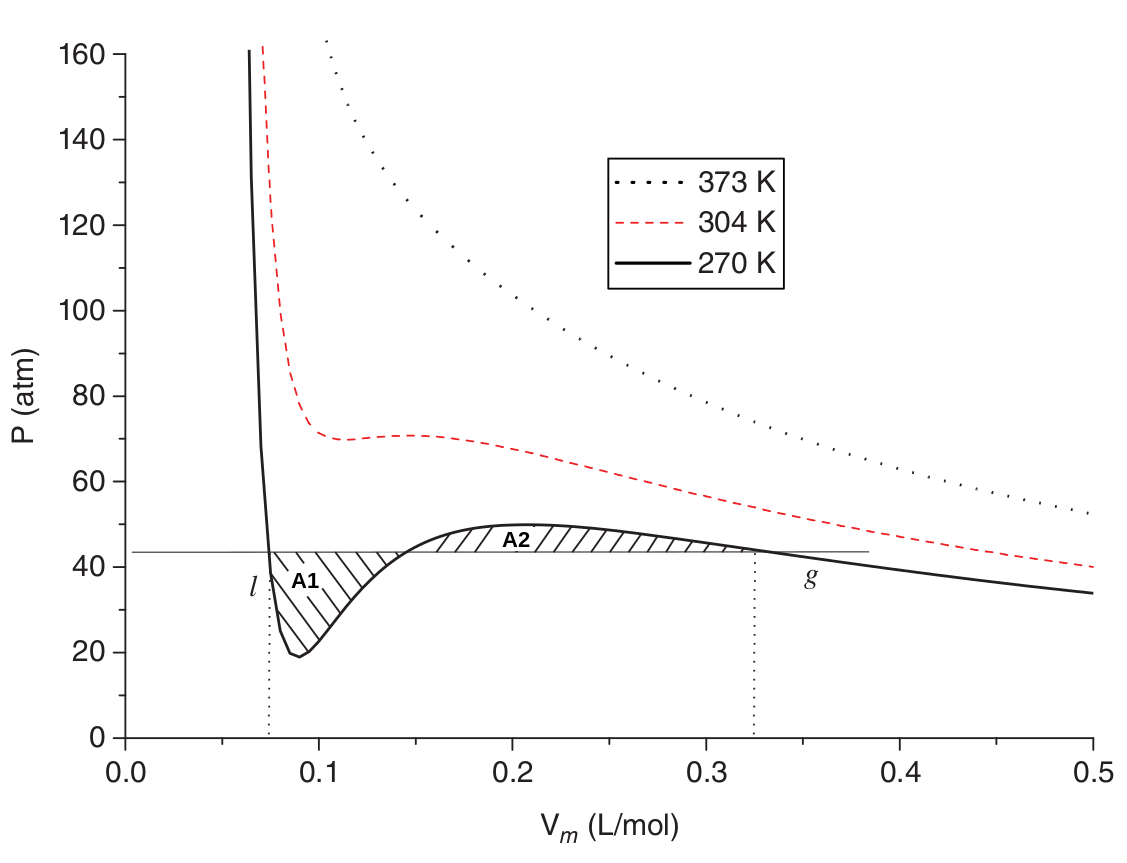
\includegraphics[width=.8\textwidth]{figs/cap4/Diagrama_P_V_del_CO2_Multiphase_LBM}
	\caption{Diagrama $P - V_m$ de la EOS de VdW del $CO_2$ con las constantes $a = 3,592$ y $b = 0,04267$, representando par a $T = 270 \> K$ los volúmenes molares del líquido y gas. \cite{huang2015multiphase}}
	\label{fig:P_V_CO2}	
\end{figure}


La Ec. (\ref{eq:VdW_P}) se puede re-estructurar como Ec. (\ref{eq:rho_eos}) puesto que $\rho = \frac{1}{v}$, siendo $v$ el volúmen másico y relacionando $V_m$ con $v$ según cada fluido. Donde para un dado valor de temperatura tendremos la coexistencia de fases con su densidad $\rho_l$ para la fase líquida y $\rho_g$ para la gaseosa.

\begin{equation*}
p_{EOS} = \frac{\rho R T}{1- \rho b} - a {\rho}^{2} \nonumber 
%\label{eq:VdW_rho}
\end{equation*}

Para un dado valor de temperatura, llamado temperatura crítica (\textit{$T_c$}) comienzan a coexistir las dos fases. En el ejemplo mostrado de la Figura \ref{fig:P_V_CO2} $T_c = 304 \> K$. Analíticamente $T_c$ surge de aplicar el criterio de la primera y segunda derivada a la Ec.(\ref{eq:rho}) como se indica en Ec.(\ref{eq:criterio_1_2_deriv}) y se deben conocer los parámetros \textit{a} y \textit{b}.

\begin{equation}
	\frac{\partial\> p}{\partial\> V_{m}} = 0 \qquad \qquad \frac{\partial^{2} \> p}{\partial\> {V_{m}}^{2}} = 0
	\label{eq:criterio_1_2_deriv}
\end{equation}

Realizando adecuadamente la adimensionalización  de la Ec.(\ref{eq:rho_eos}) se puede graficar una curva de coexistencia $T_r - \rho_r$  como se observa en la Figura \ref{fig:T_r_rho_r_analitico}, siendo $T_r = \frac{T}{T_c}$ y $\rho_r = \frac{\rho}{\rho_c}$.

\begin{figure}[h!]
	\centering
	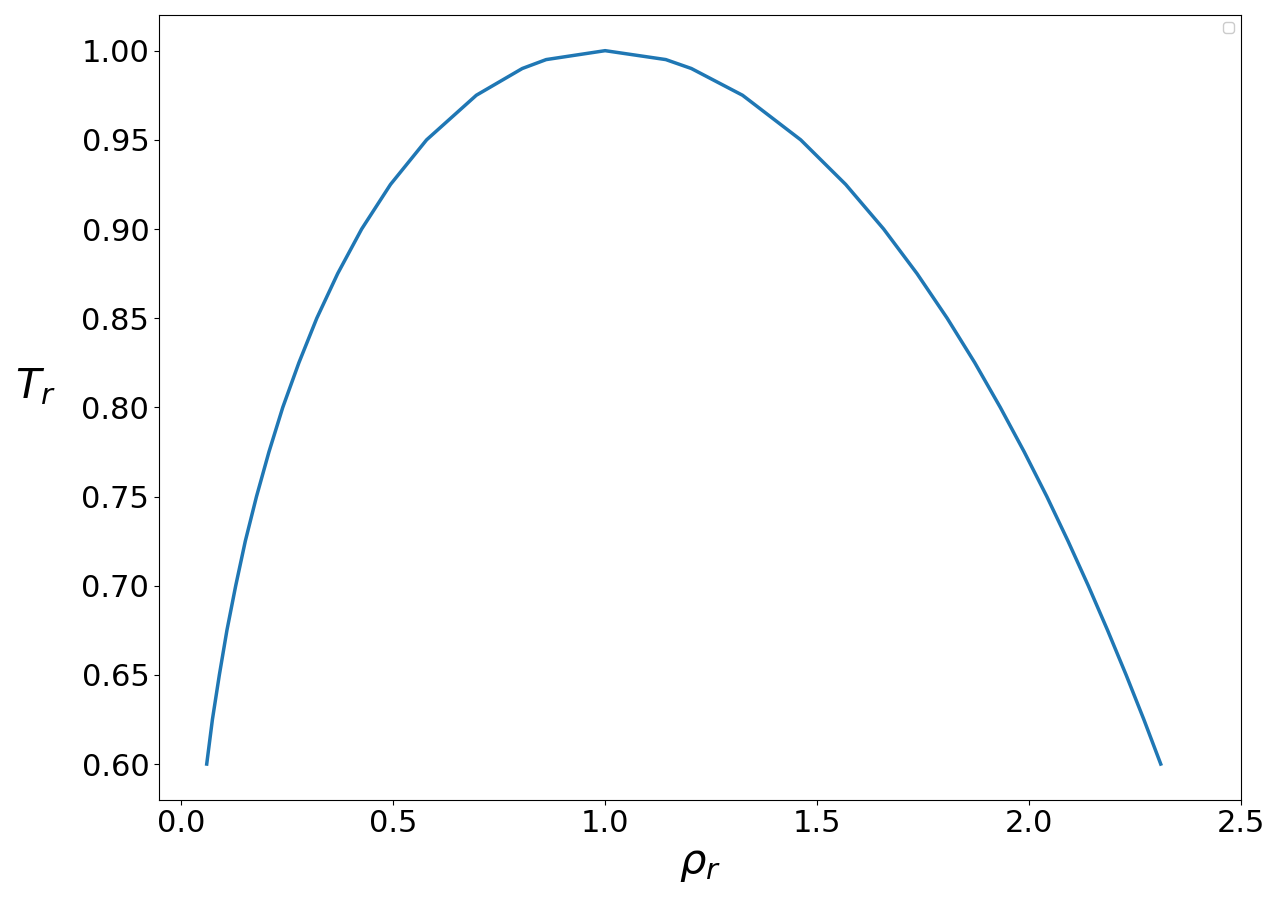
\includegraphics[width=.8\textwidth]{figs/cap4/Diagrama_T_r_vs_rho_r_analitico}
	\caption{Curva de coexistencia de fases para un fluido de VdW con los parámetros $a = 0,5 $ y $b = 4,0 $.}
	\label{fig:T_r_rho_r_analitico}	
\end{figure}

\newpage
Es de importancia destacar que las curvas de coexistencia dependen de la EOS que se esté utilizando para describir el comportamiento del fluido, en éste caso de estudio, la EOS es de VdW y posee  cómo parámetros \textit{a} y \textit{b} para describir los distintos fluidos .

\subsection{Validación}

La validación de éste problema se hizo utilizando los parámetros $a =0,5$ y $b = 4,0$; para un tamaño de malla de 201 x 201 nodos y $T_r$ variando con un paso de $0,025$ en el rango de $[0,6 - 0,975]$.  Los valores que se utilizaron de $\Lambda$ y $\mathbf{M}$ para el modelo de LBM realizado se encuentran en el Apéndice (xxxx).
%La descripción de cómo se realizó la curva de coexistencia analítica se encuentra en el Apéndice (xxxx).

La Figura(\ref{fig:v_760_MxC_c_simple}) muestra la validación del código realizado en \textbf{C} para simple precisión en una GPU NVIDIA Geforce GTX 760; con distintos parámetros $\sigma$ del modelo MRT, donde se observa que el valor de $\sigma = 0,125$ es el que mejor ajusta a la curva de coexistencia. La Figura (\ref{fig:v_760_MxC_cuda_simple}) muestra el resultados obtenidos del código realizado en \textbf{CUDA C} en simple precisión en la misma GPU.

\begin{figure}[h!]
	\centering
	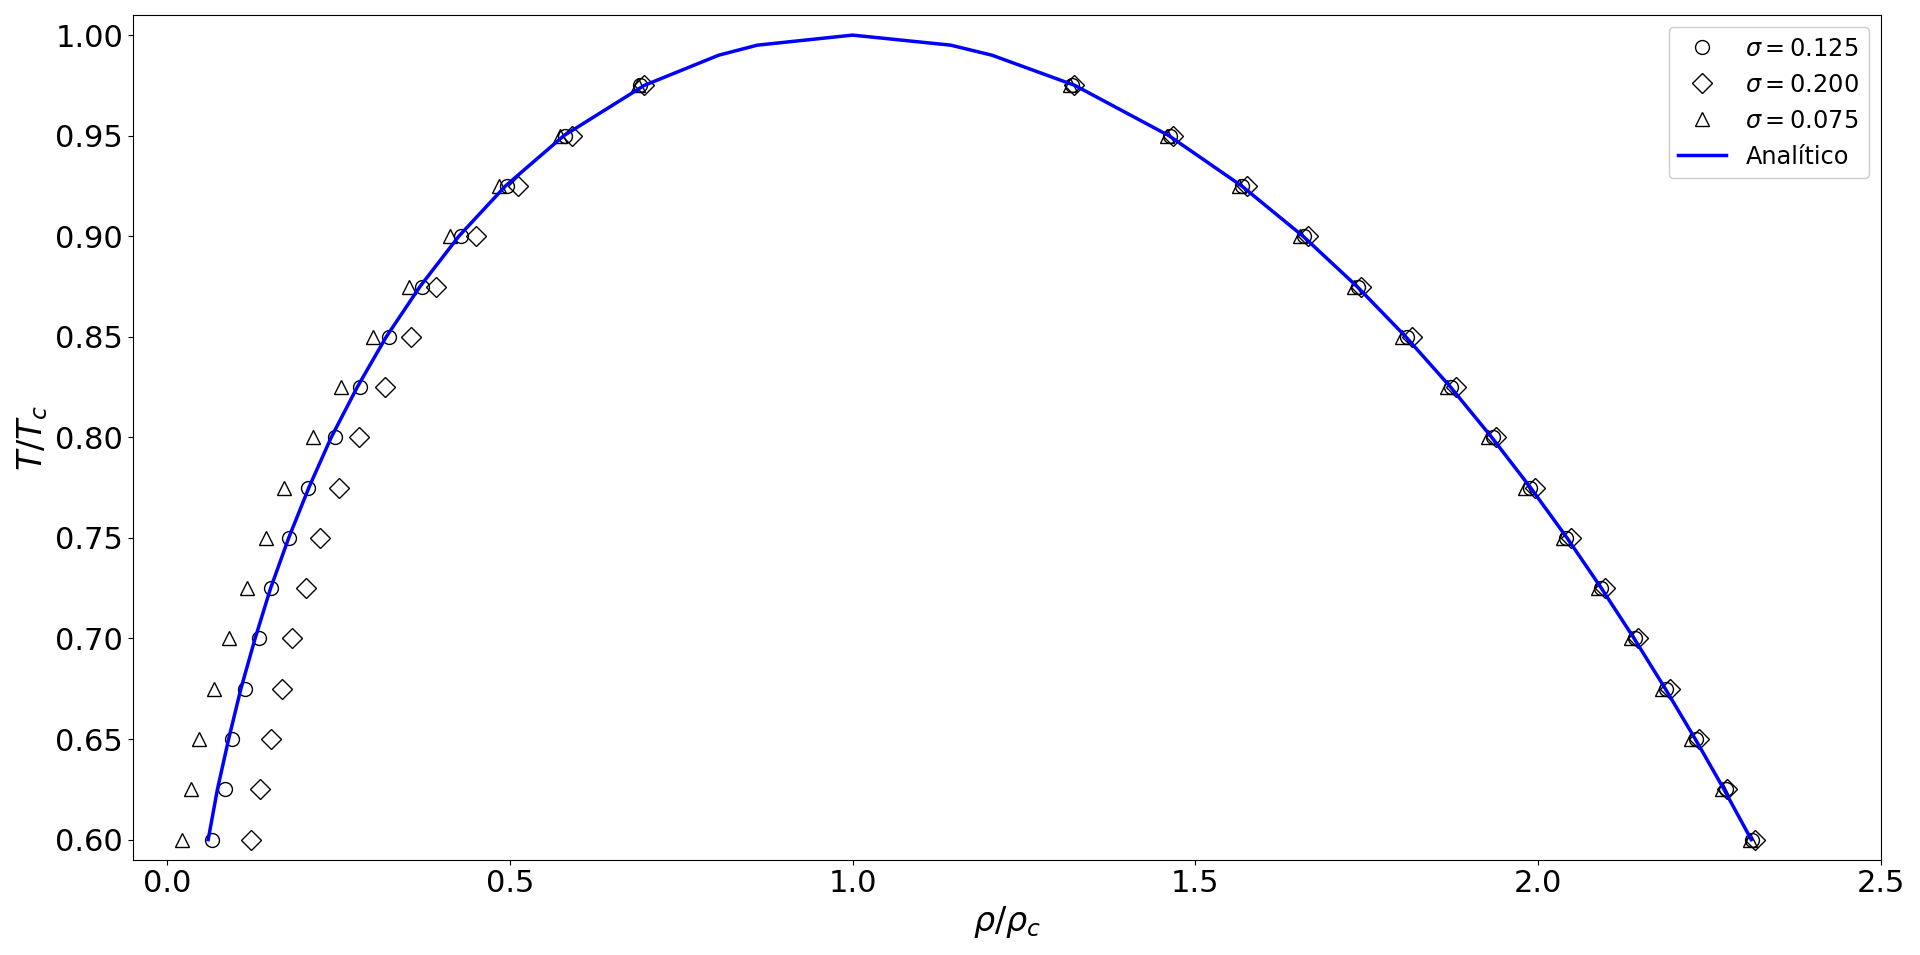
\includegraphics[width=\textwidth]{figs/cap4/v_760_MxC_c_simple}
	\caption{Curva de coexistencia de fases para un fluido de VdW con los parámetros $a = 0,5 $ y $b = 4,0 $, obtenida en simple precisión en la GPU NVIDIA Geforce GTX 760 en el código desarrollado en \textbf{C}. $\sigma = 0.075[\bigtriangleup]$	 $\sigma = 0.125[\bigcirc]$ y $\sigma = 0.200[\diamondsuit]$ }
 	\label{fig:v_760_MxC_c_simple}	
\end{figure}

\begin{figure}[h!]
	\centering
	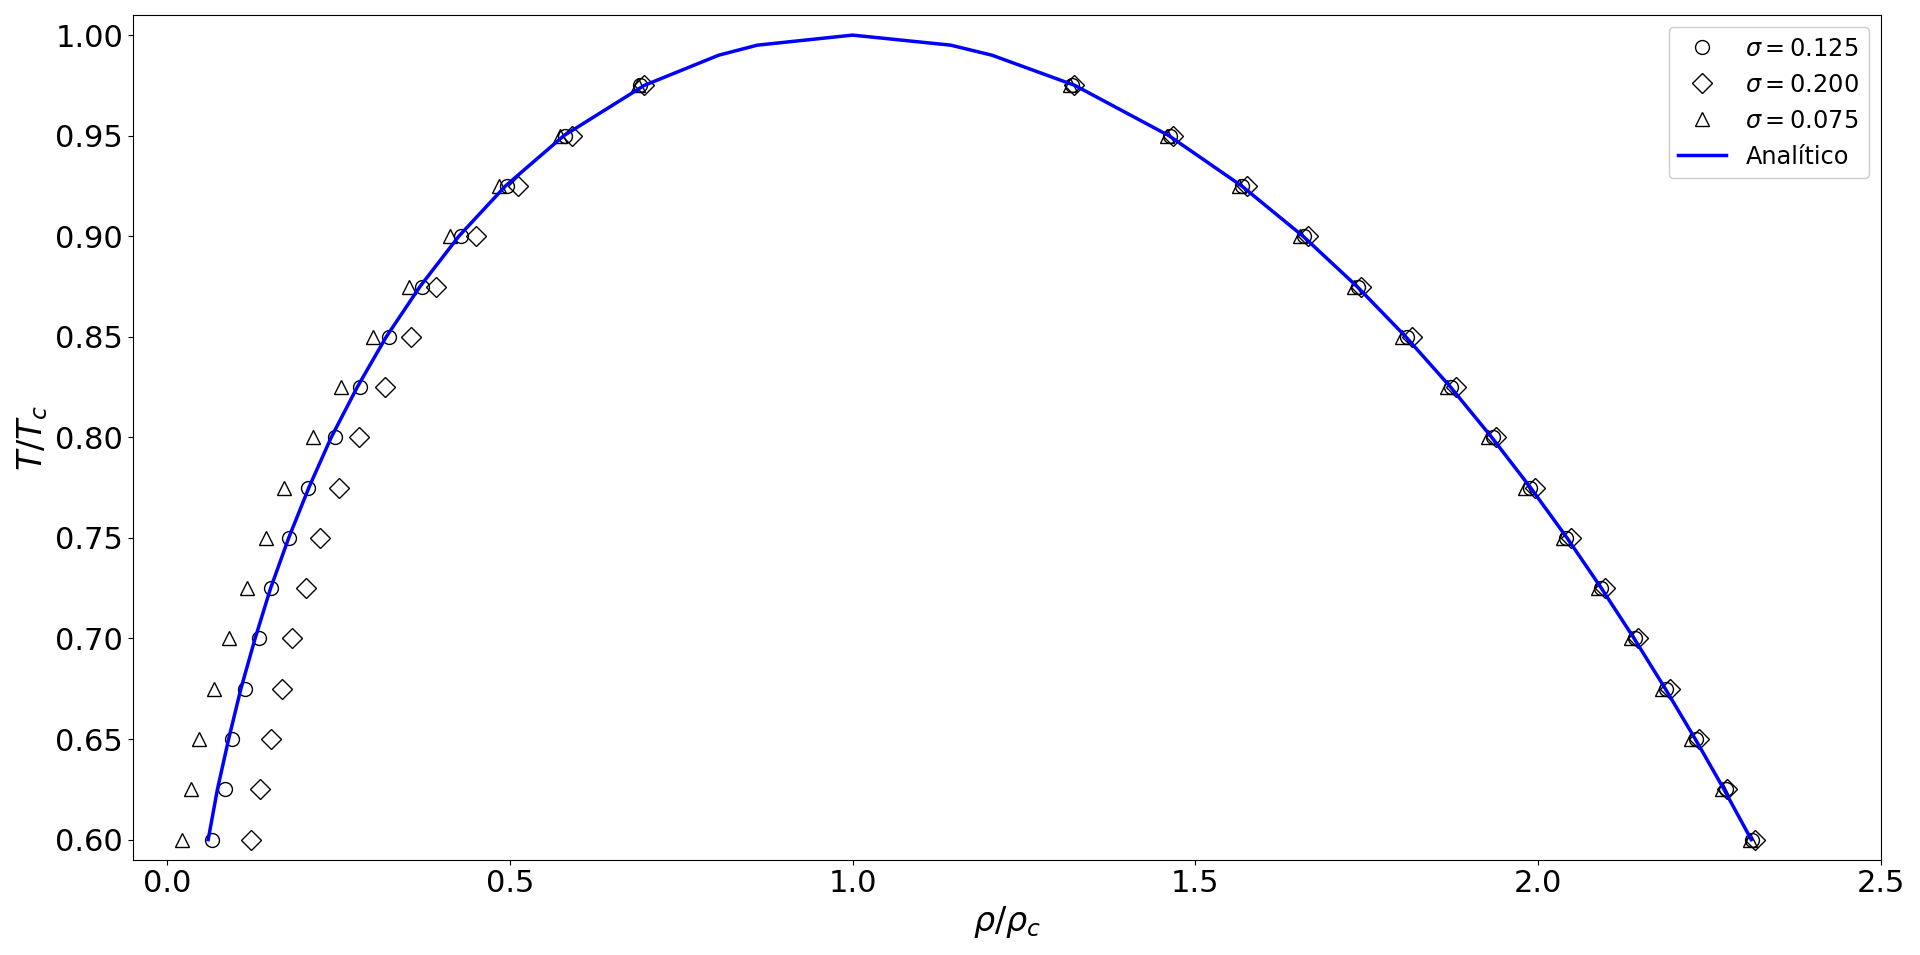
\includegraphics[width=\textwidth]{figs/cap4/v_760_MxC_cuda_simple}
	\caption{Curva de coexistencia de fases para un fluido de VdW con los parámetros $a = 0,5 $ y $b = 4,0 $, obtenida en simple precisión en la GPU NVIDIA Geforce GTX 760 en el código desarrollado en \textbf{CUDA C}. $\sigma = 0.075[\bigtriangleup]$	 $\sigma = 0.125[\bigcirc]$ y $\sigma = 0.200[\diamondsuit]$ }
	\label{fig:v_760_MxC_cuda_simple}	
\end{figure}

Ambos resultados mostrados en las Figuras (\ref{fig:v_760_MxC_c_simple}) y (\ref{fig:v_760_MxC_cuda_simple}) fueron realizados para 50000 pasos de tiempo en cada uno de los valores de $T_r$. El valor obtenido de las densidades de coexistencia de fases entre los códigos de \textbf{C} y \textbf{CUDA C} resultan exactamente iguales. 

El resultado que se obtuvo de realizar la validación en doble precisión es que los dos códigos desarrollados obtienen el mismo valor en las densidades de fase.

\newpage
\subsection{Comparación de precisiones}

En el análisis de la comparación de las precisiones, sólo se presentan los resultados obtenidos mediante el código de \textbf{C}; debido a que los resultados de \textbf{CUDA C} son idénticos.

La Figura (\ref{fig:v_760_MxC_c_comparacion}) muestra los resultados de las densidades de coexistencia de fases para simple y doble precisión, no siendo apreciable la diferencia.

\begin{figure}[h!]
	\centering
	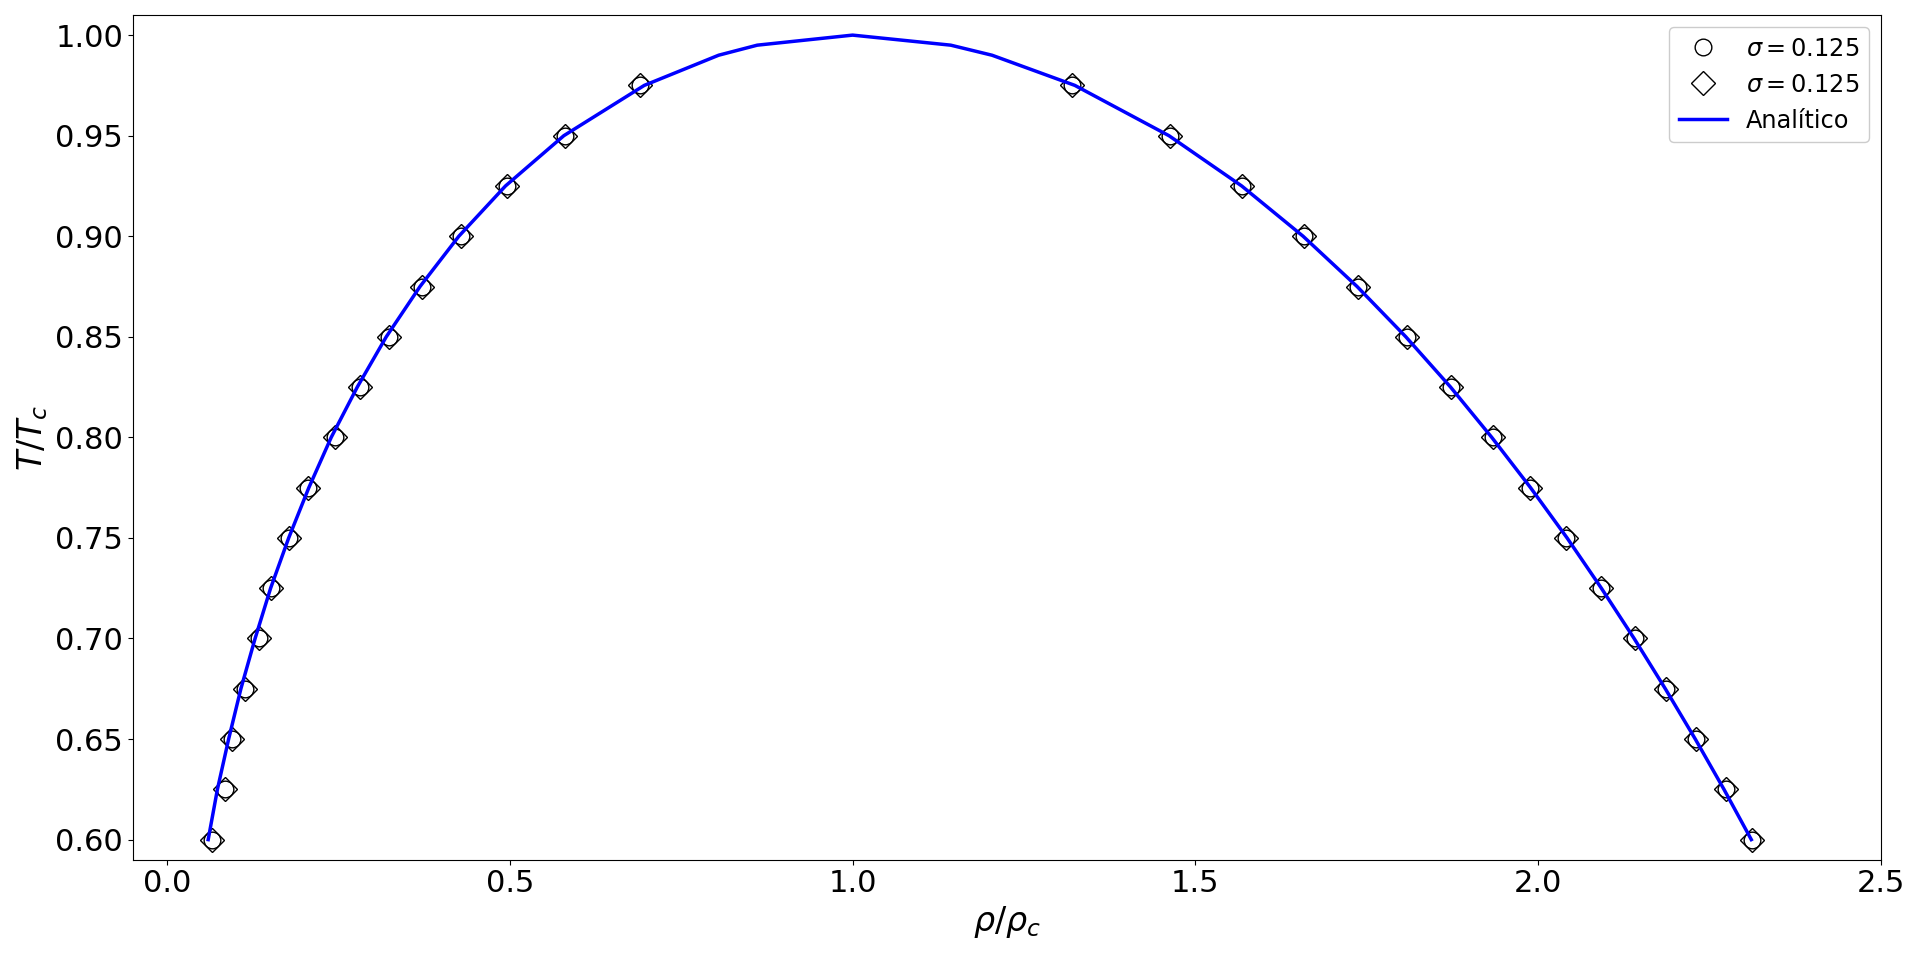
\includegraphics[width=\textwidth]{figs/cap4/v_760_MxC_c_comparacion}
	\caption{Curva de coexistencia de fases para un fluido de VdW con los parámetros $a = 0,5 $ y $b = 4,0 $, obtenida en simple precisión[$\bigcirc$] y doble precisión [$\diamondsuit$] en la GPU NVIDIA Geforce GTX 760 en el código desarrollado en \textbf{C}.} 
	\label{fig:v_760_MxC_c_comparacion}	
\end{figure}


La Tabla (\ref{tab:comp_MxC_precisiones_10}) contiene los valores de las densidades de coexistencia: analítico, y los obtenidos mediante el código en simple precisión y doble precisión. De la Figura (\ref{fig:v_760_MxC_c_comparacion}) se observa que se ajusta mejor al resultado analítico la fase líquida que la fase gaseosa, por ello la Tabla (\ref{tab:comp_MxC_precisiones_10}) presenta esta diferenciación.

Para dar una idea de proximidad a la solución analítica se adoptó como parámetro la distancia entre los vectores de densidad de fase obtenido y el analítico. La distancia se calculó por medio de la Norma Euclídea, siendo calculada la distancia entre dos vectores \textbf{\textit{A}} y \textbf{\textit{B}} con \textit{i} elementos como indica la Ec.(\ref{eq:norma_euclidea}):

\begin{align}
dist(\mathbf{A},\mathbf{B}) = \sqrt{\sum_i {\left( a_i - b_i \right)}^2  }
\label{eq:norma_euclidea}
\end{align}

Los resultados que muestra la Tabla (\ref{tab:comp_MxC_precisiones_10}) en cuanto a la distancia de los vectores se observa que en doble precisión los resultados se aproximan mejor en la densidad de coexistencia de la fases, en la fase gaseosa; mientras que para la densidad de coexistencia de fase, de la fase líquida, se aproxima mejor mediante simple precisión. 

Porcentualmente para la fase gaseosa, la distancia calculada en simple precisión es 0,0034 \% mayor que en doble precisión; para la fase líquida la distancia en doble precisión es 0,0491 \% mayor que en simple precisión.


% Please add the following required packages to your document preamble:
% \usepackage{multirow}
\begin{table}[h!]
\centering
%\resizebox{17cm}{!}{
	\begin{tabular}{|c|c|c|c|c|c|c|}
	\hline
	& \multicolumn{3}{c|}{${\rho_{r}}_{\>gaseoso}$}      & \multicolumn{3}{c|}{${\rho_{r}}_{\>líquido}$} \\ \hline
	$\mathbf{T_r}$    & \textbf{Analítico}      & \textbf{Simple}       & \textbf{Doble}     & \textbf{Analítico}      & \textbf{Simple}     & \textbf{Doble}   \\ \hline
	0.600 & 0.0599097 & 0.0653772 & 0.0653724 & 1.32424  & 1.31956 & 1.31975 \\ \hline
	0.625 & 0.0733723 & 0.0848112 & 0.0847656 & 1.46149  & 1.46239 & 1.4624  \\ \hline
	0.650 & 0.0897449 & 0.0951336 & 0.095124  & 1.56762  & 1.56858 & 1.56859 \\ \hline
	0.675 & 0.107606  & 0.113153  & 0.113147  & 1.56762  & 1.65819 & 1.65821 \\ \hline
	0.700 & 0.128332  & 0.13353   & 0.133511  & 1.6572   & 1.73703 & 1.73704 \\ \hline
	0.725 & 0.150966  & 0.15182   & 0.151811  & 1.73595  & 1.80812 & 1.80813 \\ \hline
	0.750 & 0.177353  & 0.177323  & 0.177319  & 1.80706  & 1.87326 & 1.87328 \\ \hline
	0.775 & 0.206739  & 0.206086  & 0.206075  & 1.87233  & 1.93364 & 1.93364 \\ \hline
	0.800 & 0.23938   & 0.244229  & 0.244223  & 1.93243  & 1.98754 & 1.98759 \\ \hline
	0.825 & 0.277393  & 0.281299  & 0.281284  & 1.98899  & 2.04083 & 2.04085 \\ \hline
	0.850 & 0.319677  & 0.323471  & 0.323456  & 2.0423   & 2.09124 & 2.09124 \\ \hline
	0.875 & 0.368925  & 0.371915  & 0.371891  & 2.09234  & 2.14114 & 2.14117 \\ \hline
	0.900 & 0.425549  & 0.428416  & 0.428335  & 2.14012  & 2.18665 & 2.18665 \\ \hline
	0.925 & 0.493618  & 0.495973  & 0.495947  & 2.18563  & 2.23017 & 2.23019 \\ \hline
	0.950 & 0.493618  & 0.580402  & 0.580368  & 2.22933  & 2.27407 & 2.27411 \\ \hline
	0.975 & 0.578746  & 0.690126  & 0.690247  & 2.27117  & 2.312   & 2.312   \\ \hline
	\textbf{Distancia} & -         & 2.05233   & 2.05226   & -        & 0.14234 & 0.14241 \\ \hline
\end{tabular}%}
    \caption{Comparación de las precisiones con respecto a cuánto se acercan al valor analitico, tanto para doble, como simple precision, la norma utilizada para medir la distancia de los vectores es la norma  euclídea. Para el problema de la Construcción de Maxwell con la GPU NVIDIA Geforce GTX 760.}
    \label{tab:comp_MxC_precisiones_10}
    \end{table}



\newpage

\subsection{Speed Up}

En la presente sección se muestran las mejora en el tiempo de cálculo realizados para el código de \textbf{C} y \textbf{CUDA C}. La comparación se realizó en simple y doble precisión; en dos GPU, siendo las mismas NVIDIA Geforce GTX 760 y NVIDIA Geforce GTX 970. Se tomó una $T_r$ fija y se varió el tamaño de la grilla, de manera que ésta siempre fuese cuadrada, respetando un número de nodos de potencia de 2 en los lados del cuadrado. La cantidad de \textit{thread blocks} que se utilizó para realizar la comnparación en el código de \textbf{CUDA} fueron de potencia de 2.

\subsubsection{NVIDIA Geforce GTX 760}

Los tamaños de grilla que se utilizaron para realizar las pruebas de tiempo de ésta placa, tienen el rango de grilla de 16x16 nodos hasta 2048x2048 nodos. La cantidad de \textit{thread blocks} que se utilizó fueron de 1 a 512.

Las Figuras (\ref{fig:s_760_MxC_simple_1.0}) y (\ref{fig:s_760_MxC_double_1.0}) muestran el \textit{Speed Up} obtenido comparando los códigos de \textbf{C} y \textbf{CUDA C}, donde la Figura (\ref{fig:s_760_MxC_simple_1.0}) está obtenida con simple precisión y la Figura (\ref{fig:s_760_MxC_double_1.0}) en doble precisión. El mejor resultado en ambos casos se obtuvo para un número de \textit{thread block} igual a 64, donde la mejora fue de 18.67 y 11.40 en simple y doble precisión respectivamente, para el mayor número de elementos de malla.


\begin{figure}[h!]
	\centering
	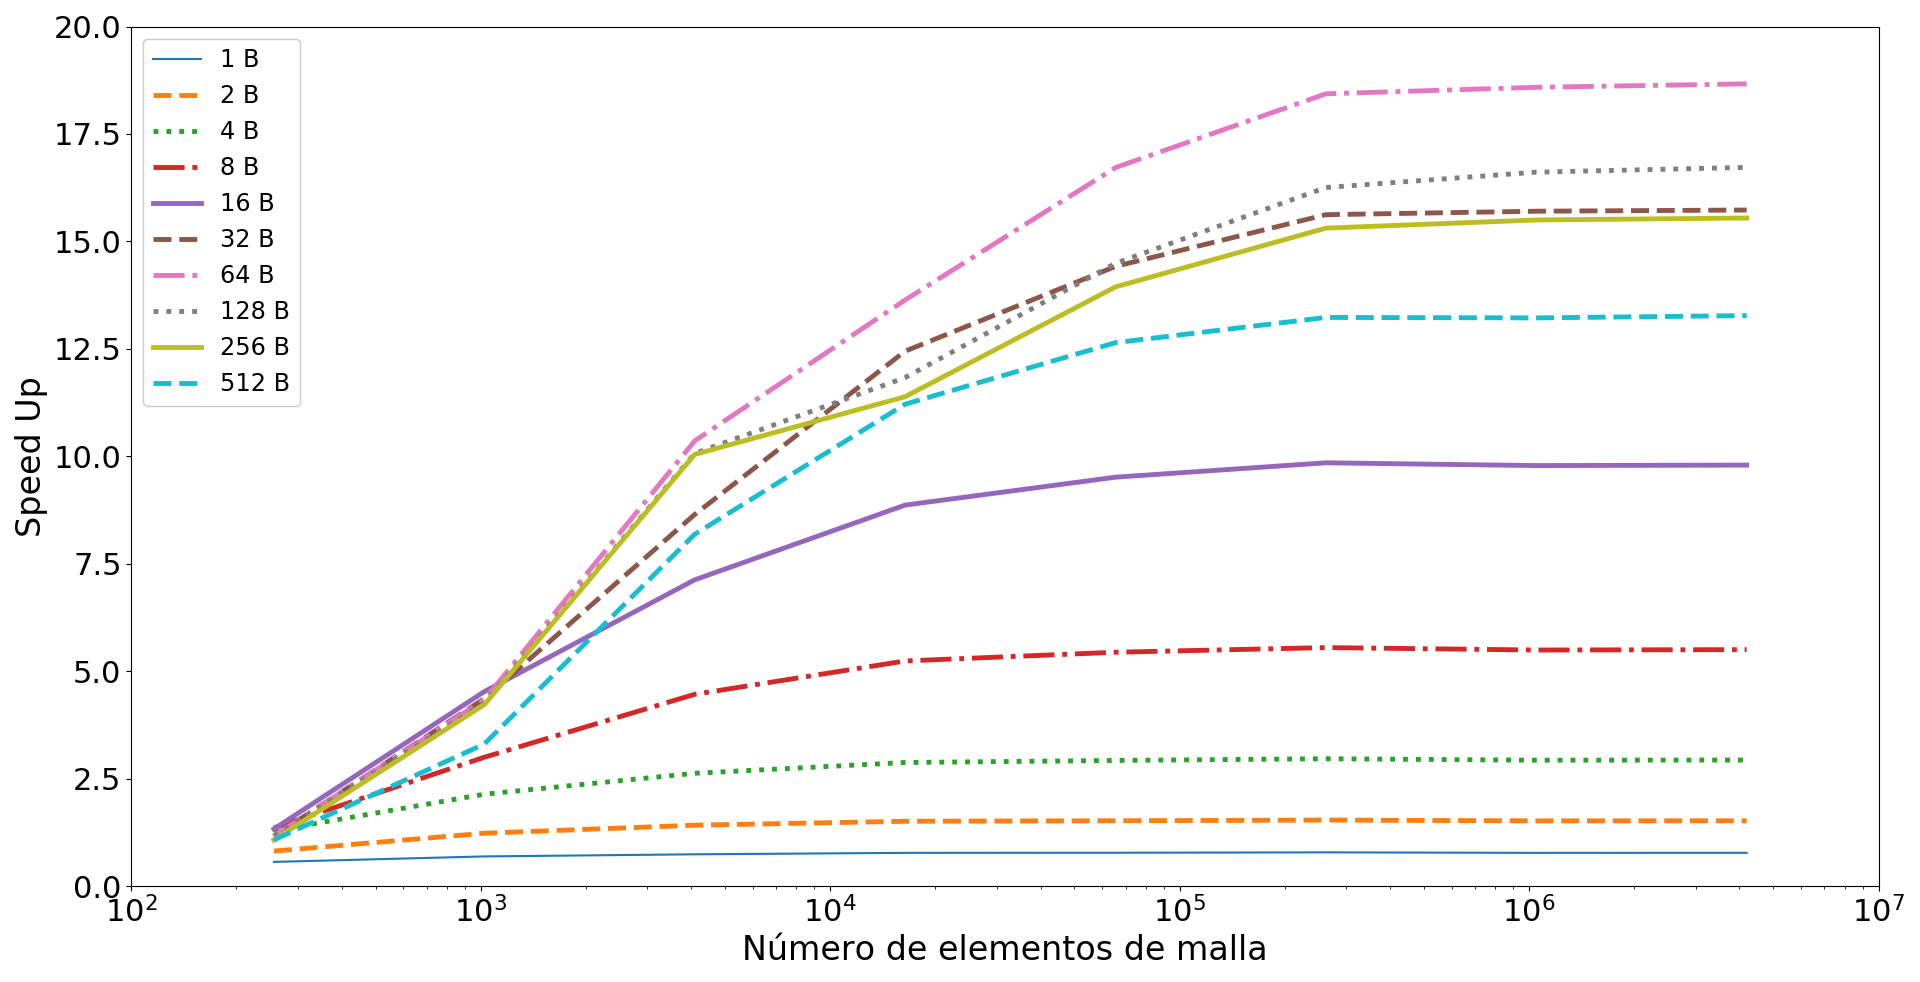
\includegraphics[width=\textwidth]{figs/cap4/s_760_MxC_simple_10}
	\caption{Speed Up realizado para el problema de la Construcción de Maxwell con la GPU NVIDIA Geforce GTX 760 en simple precisión, comparando los códigos de \textbf{C} y \textbf{CUDA C}.} 
	\label{fig:s_760_MxC_simple_1.0}	
\end{figure}

\begin{figure}[h!]
	\centering
	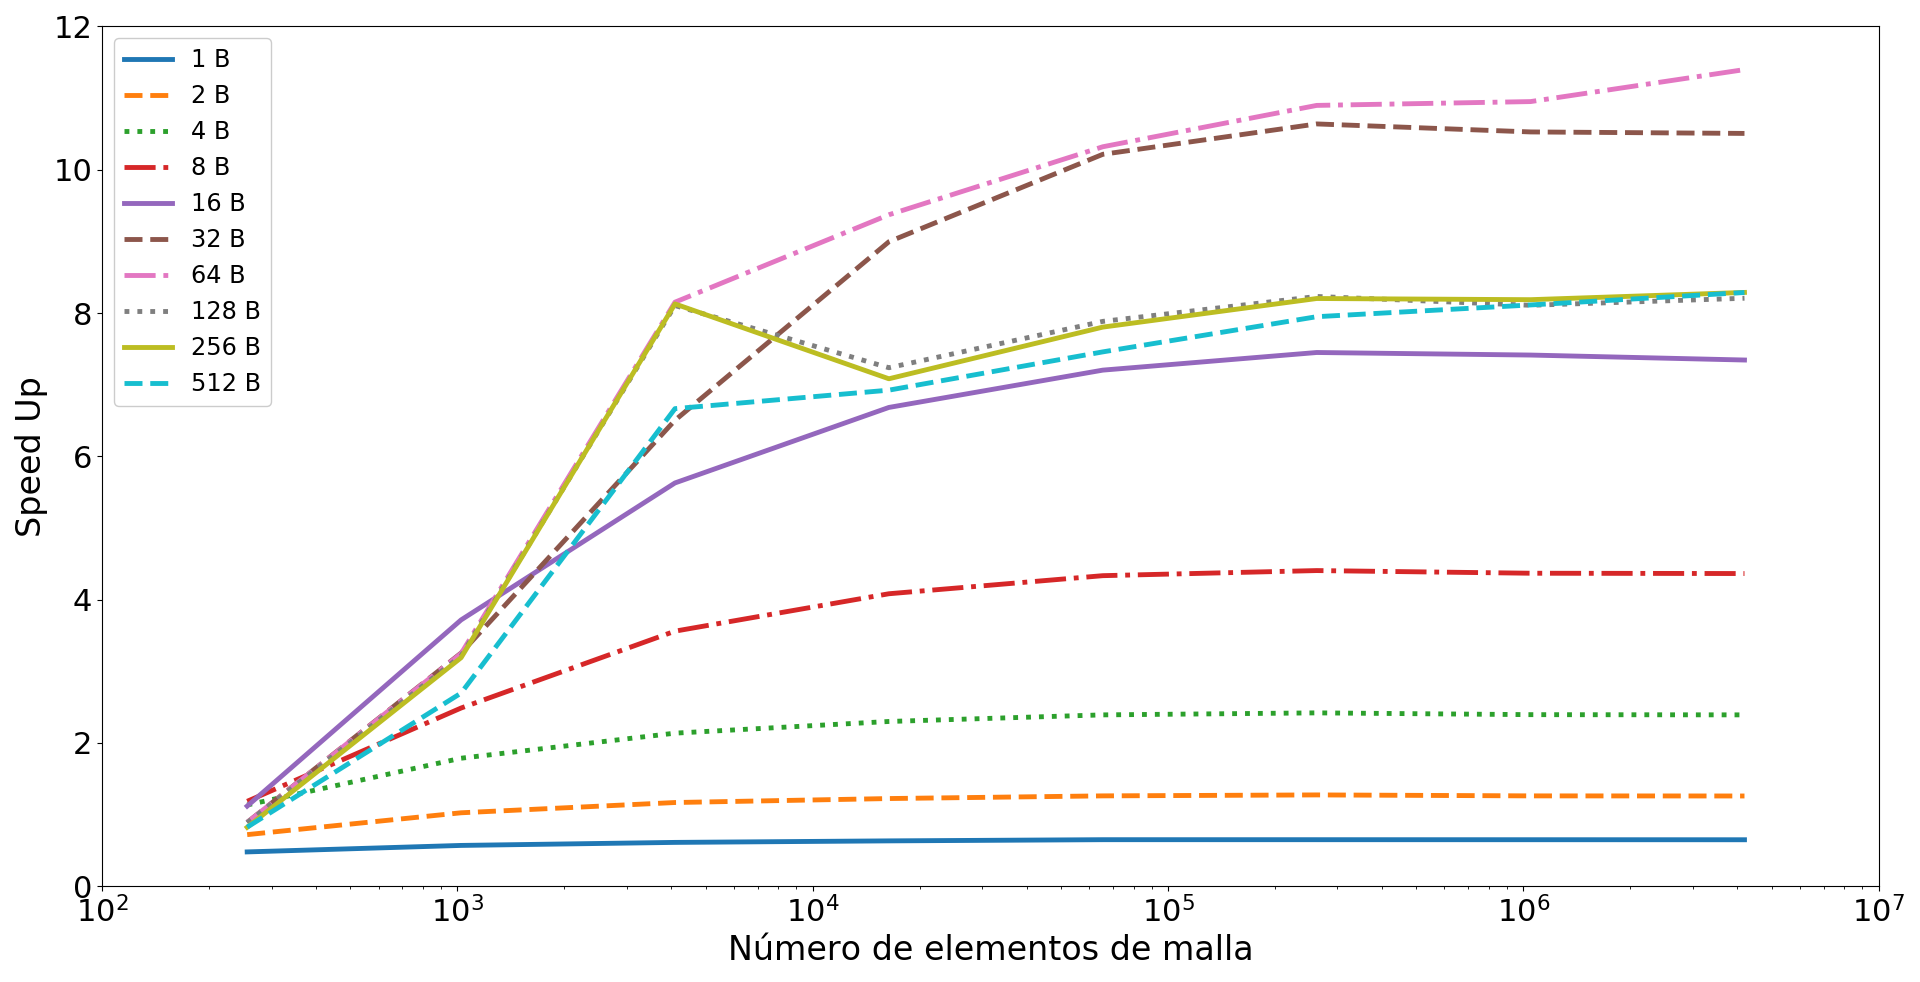
\includegraphics[width=\textwidth]{figs/cap4/s_760_MxC_double_10}
	\caption{Speed Up realizado para el problema de la Construcción de Maxwell con la GPU NVIDIA Geforce GTX 760 en doble precisión, comparando los códigos de \textbf{C} y \textbf{CUDA C}.} 
	\label{fig:s_760_MxC_double_1.0}	
\end{figure}

\newpage

Las Figuras (\ref{fig:c_760_MxC_c_10}) y (\ref{fig:c_760_MxC_cuda_10}) muestran el \textit{Speed Up} obtenido comparando simple precisión y doble precisión, donde la Figura (\ref{fig:c_760_MxC_c_10}) está obtenida el código de \textbf{C} y la Figura (\ref{fig:c_760_MxC_cuda_10}) en el código de \textbf{CUDA C}. 

En el código de \textbf{C} para el mayor número de elementos de la malla, el resultado de tiempos de cálculo en doble precisión es apenas 1,026 veces mayor que en  simple precisión. En contraste, al fijarse el resultado para un número de \textit{thread block} igual a 64 (el que mayor ganancia obtuvo), el tiempo de cálculo en doble precisión es 1,68 veces mayor que en simple precisión; para el mayor número de elementos de malla calculado.

\begin{figure}[h!]
	\centering
	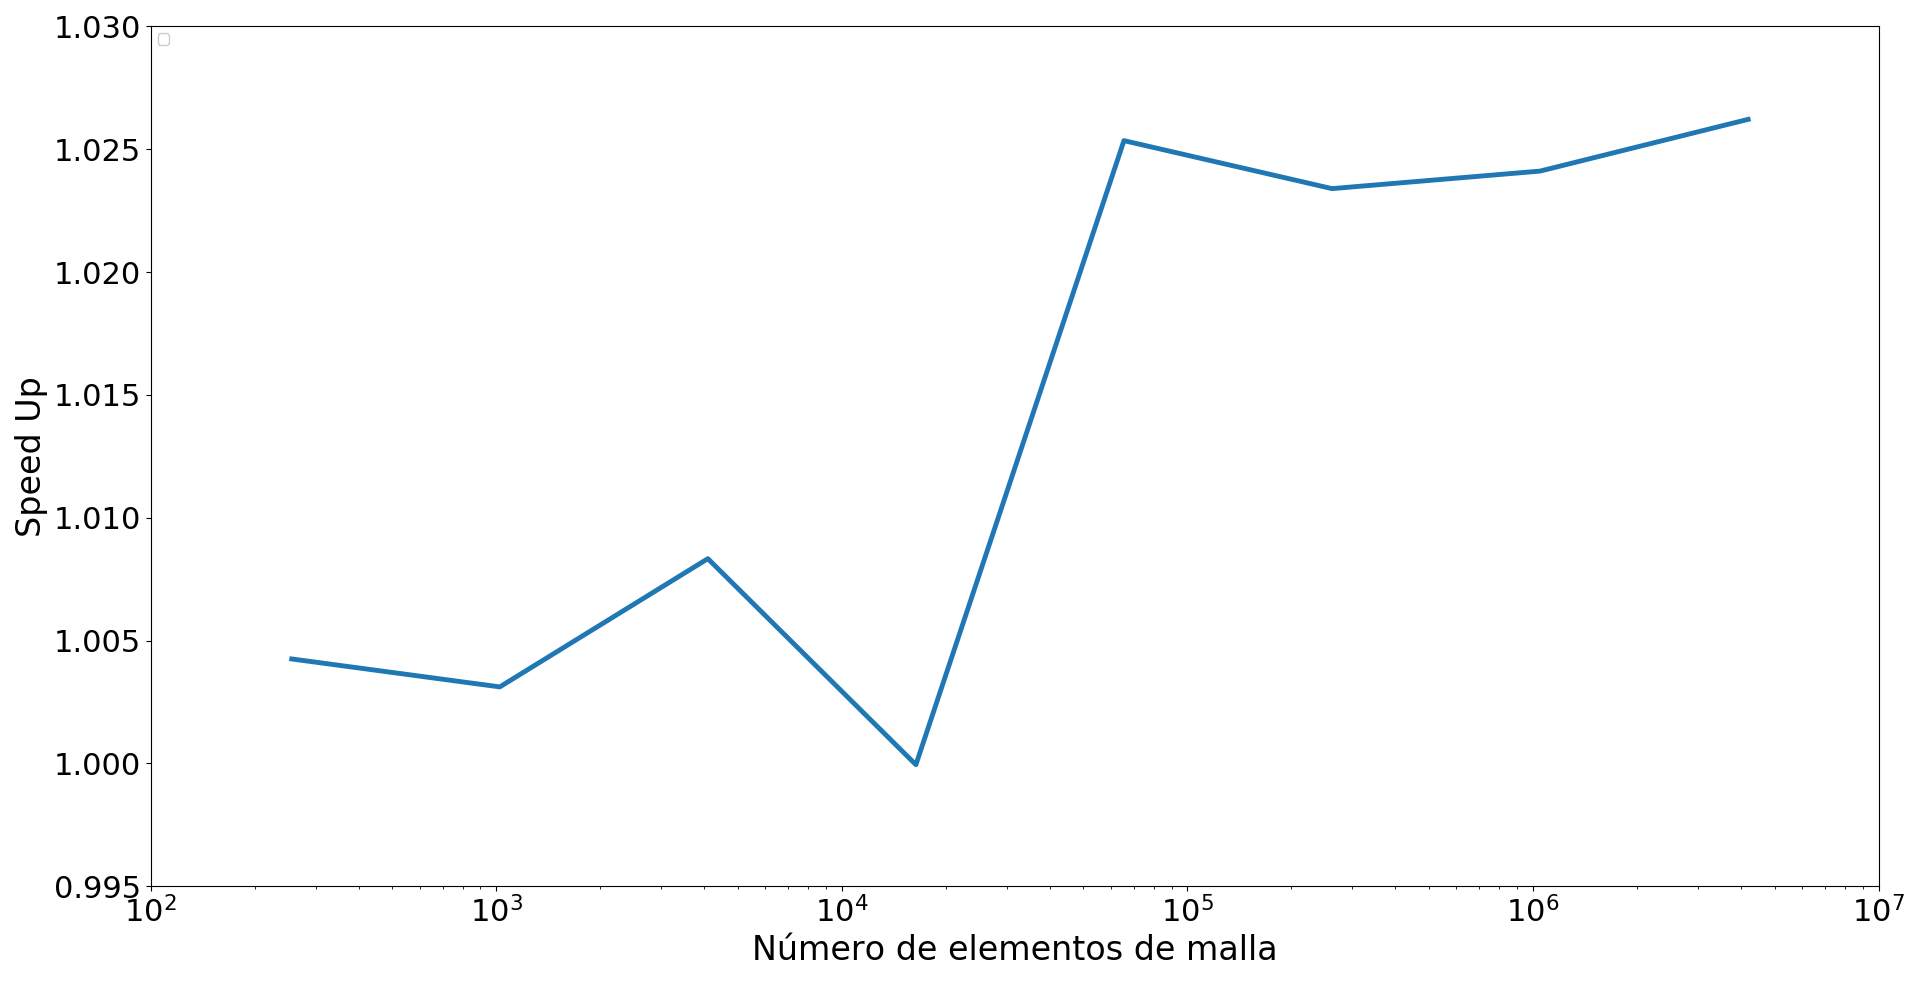
\includegraphics[width=\textwidth]{figs/cap4/c_760_MxC_c_10}
	\caption{Speed Up realizado para el problema de la Construcción de Maxwell con la GPU NVIDIA Geforce GTX 760 en en el código de \textbf{C}, comparando simple precisión y doble precisión.} 
	\label{fig:c_760_MxC_c_10}	
\end{figure}

\begin{figure}[h!]
	\centering
	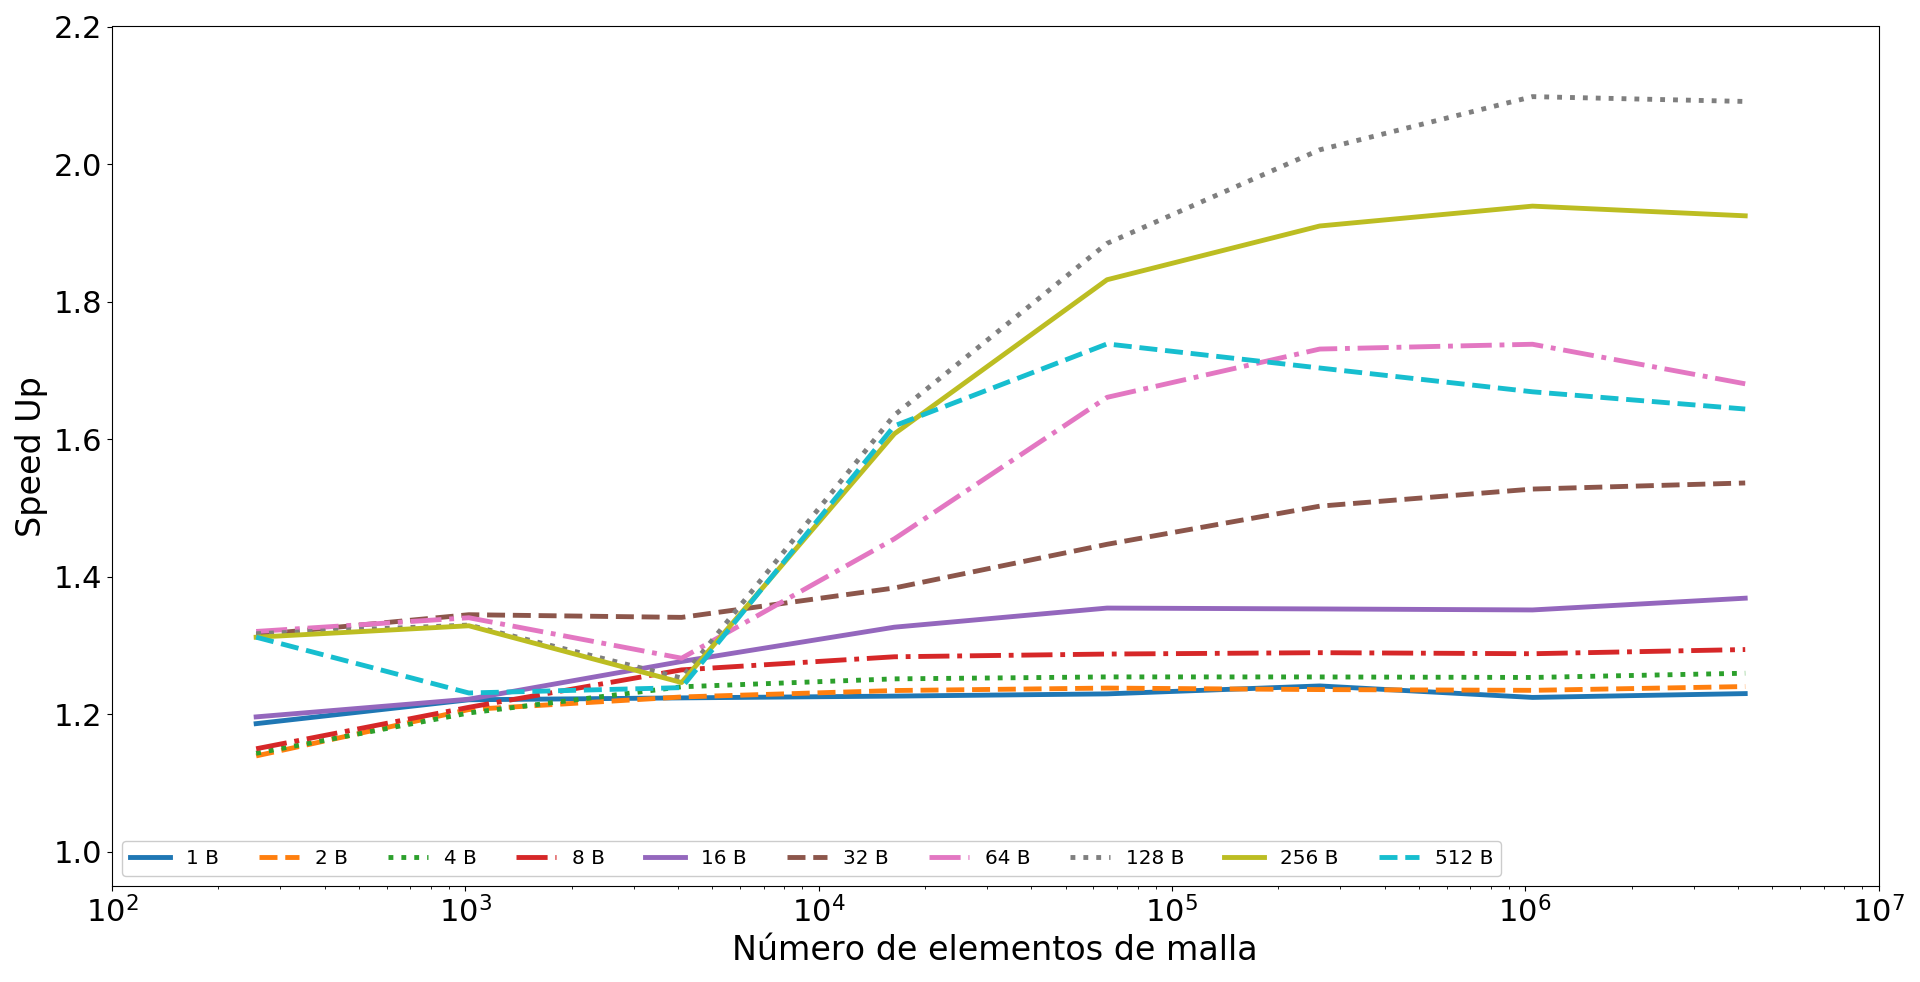
\includegraphics[width=\textwidth]{figs/cap4/c_760_MxC_cuda_10}
	\caption{Speed Up realizado para el problema de la Construcción de Maxwell con la GPU NVIDIA Geforce GTX 760 en en el código de \textbf{CUDA C}, comparando simple precisión y doble precisión.} 
	\label{fig:c_760_MxC_cuda_10}	
\end{figure}

Los valores que se obtuvieron en las Figuras (\ref{fig:s_760_MxC_simple_1.0}), (\ref{fig:s_760_MxC_double_1.0}), (\ref{fig:c_760_MxC_c_10}) y (\ref{fig:c_760_MxC_cuda_10}) se encuentran en el Apéndice \ref{apend_MxC_760}

\newpage

\subsubsection{NVIDIA Geforce GTX 970}

Los tamaños de grilla que se utilizaron para realizar las pruebas de tiempo de ésta placa, tienen el rango de grilla de 16x16 nodos hasta 4096x4096 nodos en simple precisión y de 16x16 nodos hasta 2048x2048 nodos en doble precisión . La cantidad de \textit{thread blocks} que se utilizó fueron de 1 a 512.

Las Figuras (\ref{fig:s_970_MxC_simple_10}) y (\ref{fig:s_970_MxC_double_10}) muestran el \textit{Speed Up} obtenido comparando los códigos de \textbf{C} y \textbf{CUDA C}, donde la Figura (\ref{fig:s_970_MxC_simple_10}) está obtenida con simple precisión y la Figura (\ref{fig:s_970_MxC_double_10}) en doble precisión. El mejor resultado en ambos casos se obtuvo para un número de \textit{thread block} igual a 32, donde la mejora fue de 23.39 y 10.96 en simple y doble precisión respectivamente, para el mayor número de elementos de malla.

Las Figuras (\ref{fig:c_970_MxC_c_10}) y (\ref{fig:c_970_MxC_cuda_10}) muestran el \textit{Speed Up} obtenido comparando simple precisión y doble precisión, donde la Figura (\ref{fig:c_970_MxC_c_10}) está obtenida el código de \textbf{C} y la Figura (\ref{fig:c_970_MxC_cuda_10}) en el código de \textbf{CUDA C}.

En el código de \textbf{C} para el mayor número de elementos de la malla, el resultado de tiempos de cálculo en doble precisión es apenas 1,035 veces mayor que en  simple precisión. En contraste, al fijarse el resultado para un número de \textit{thread block} igual a 32 (el que mayor ganancia obtuvo), el tiempo de cálculo en doble precisión es 1,29 veces mayor que en simple precisión; para el mayor número de elementos de malla calculado.

\begin{figure}[h!]
	\centering
	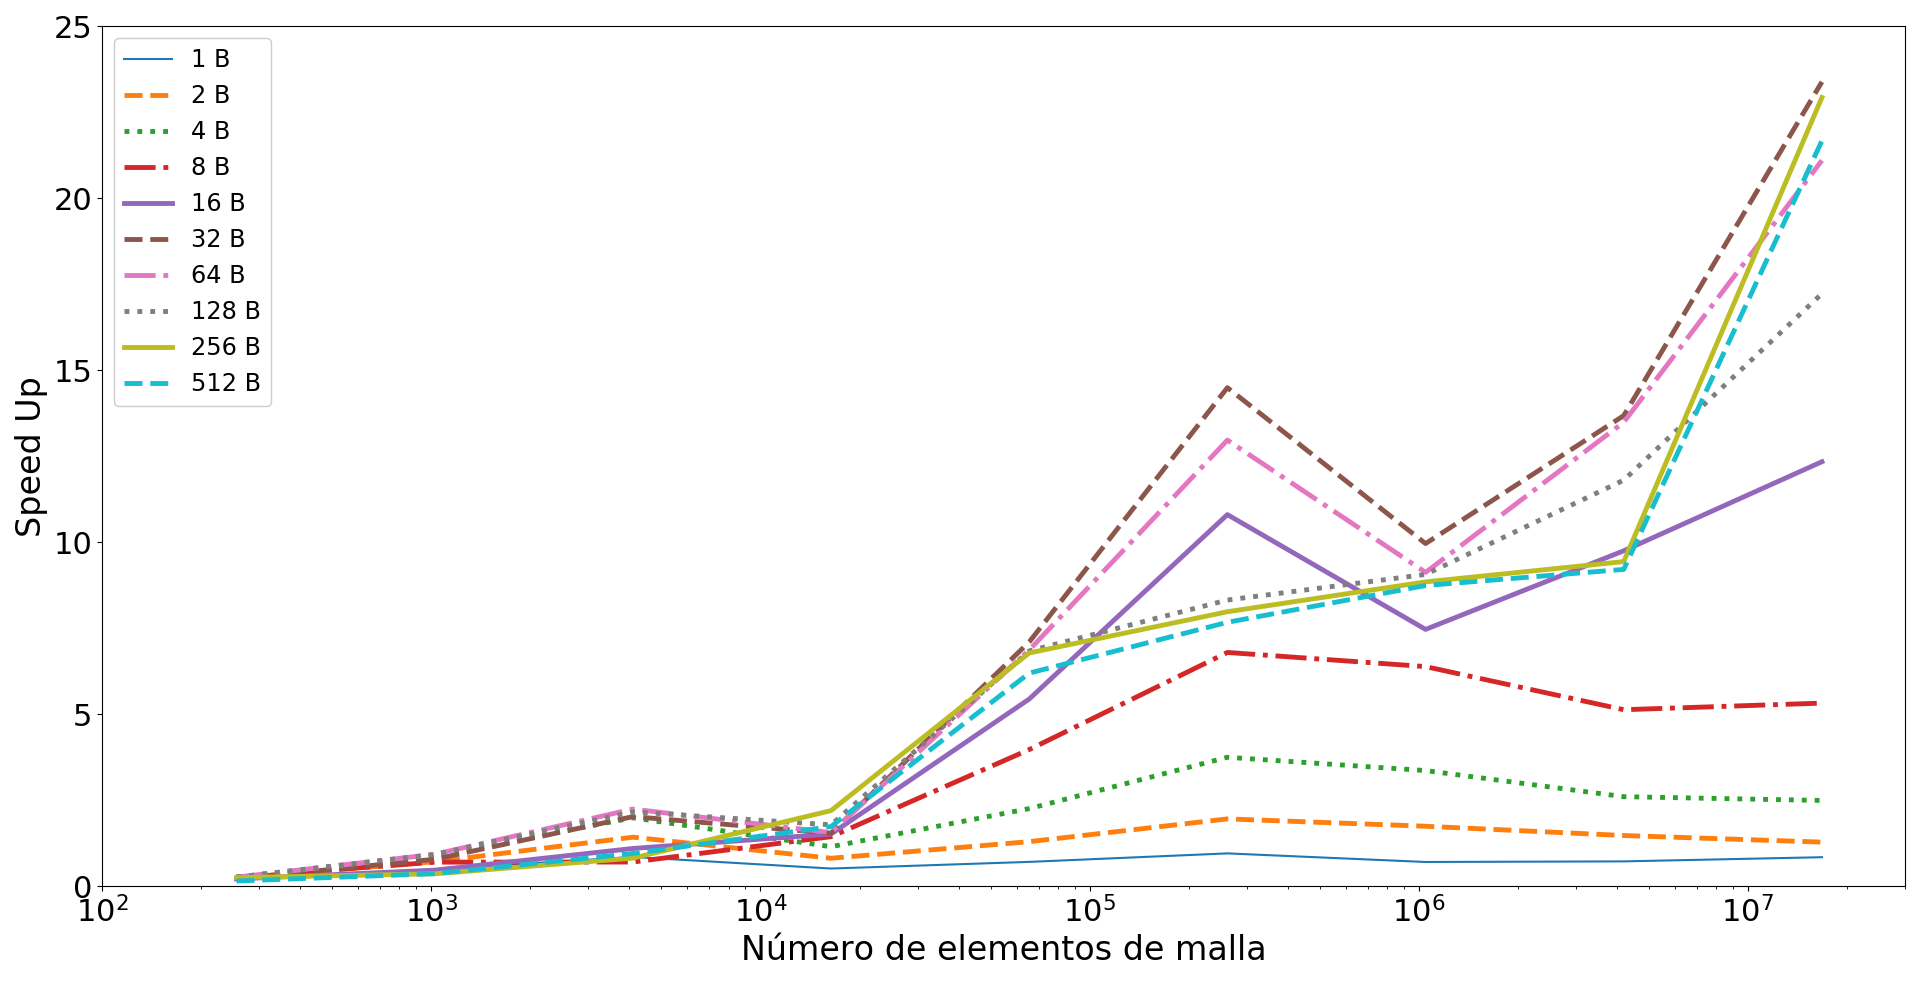
\includegraphics[width=\textwidth]{figs/cap4/s_970_MxC_simple_10}
	\caption{Speed Up realizado para el problema de la Construcción de Maxwell con la GPU NVIDIA Geforce GTX 970 en simple precisión, comparando los códigos de \textbf{C} y \textbf{CUDA C}.} 
	\label{fig:s_970_MxC_simple_10}	
\end{figure}

\begin{figure}[h!]
	\centering
	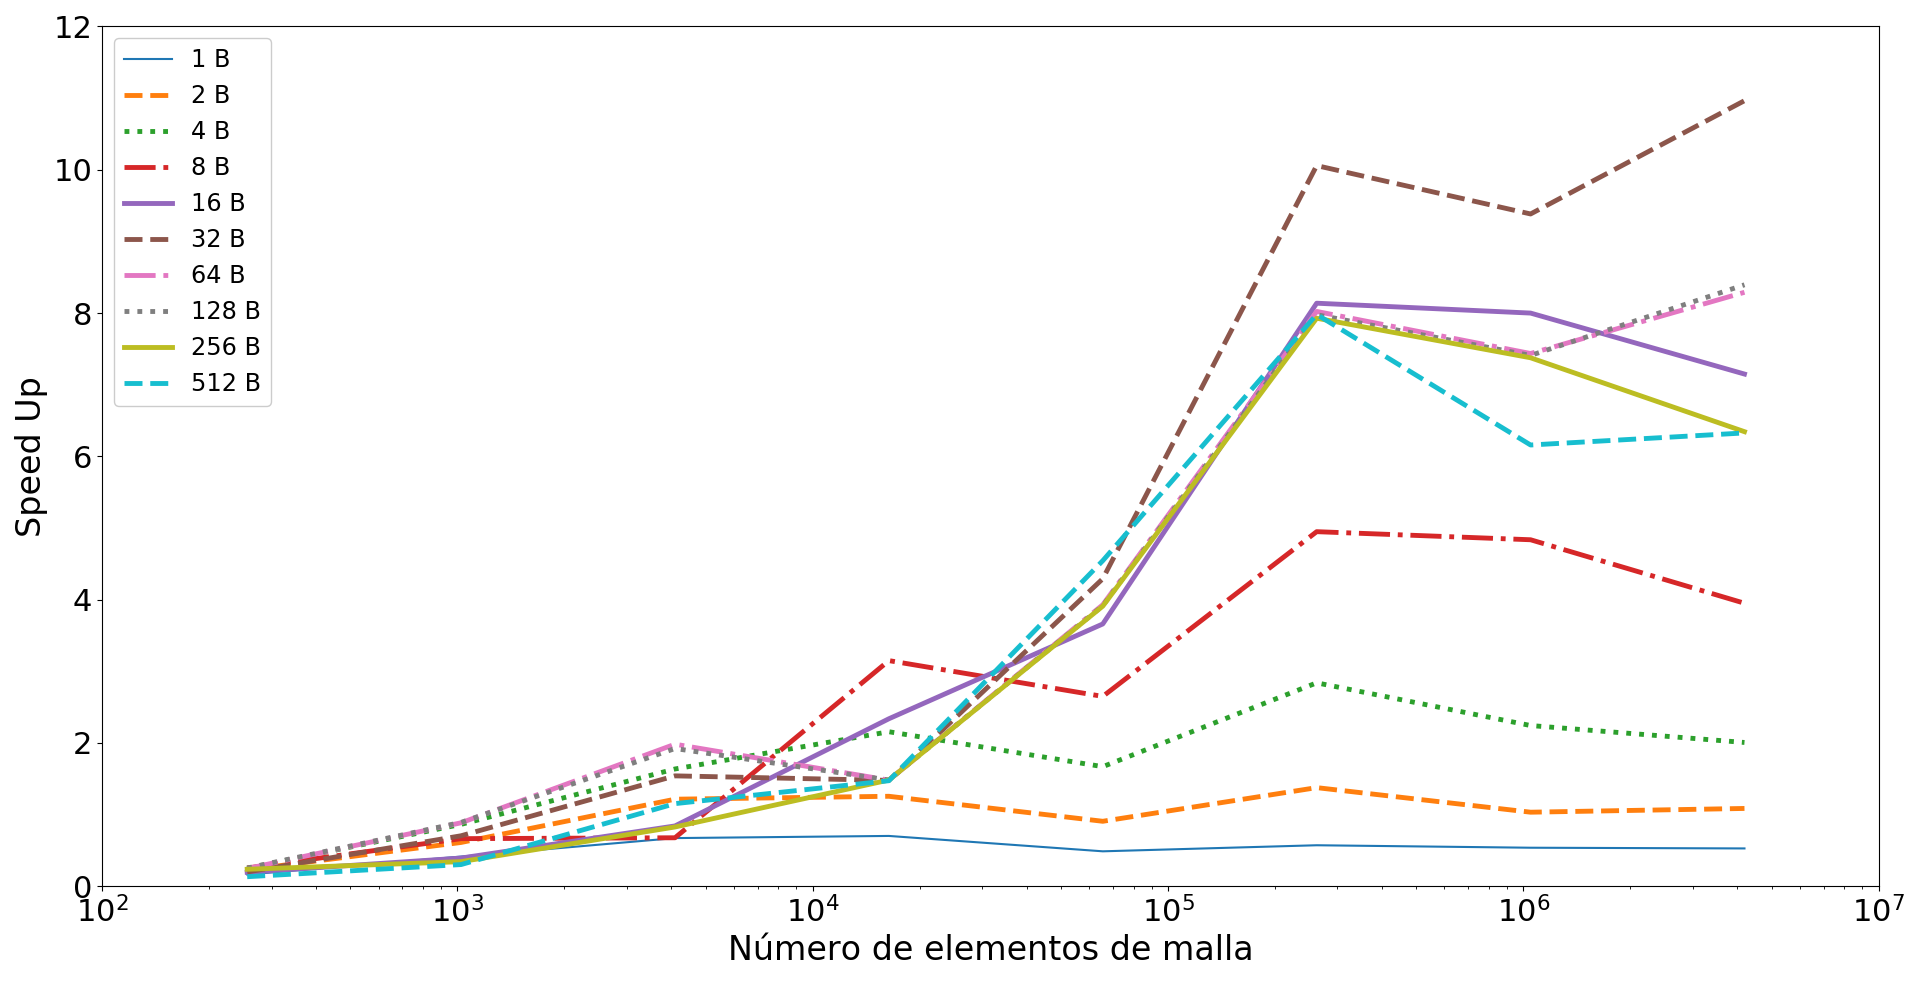
\includegraphics[width=\textwidth]{figs/cap4/s_970_MxC_double_10}
	\caption{Speed Up realizado para el problema de la Construcción de Maxwell con la GPU NVIDIA Geforce GTX 970 en doble precisión, comparando los códigos de \textbf{C} y \textbf{CUDA C}.} 
	\label{fig:s_970_MxC_double_10}	
\end{figure}


\begin{figure}[h!]
	\centering
	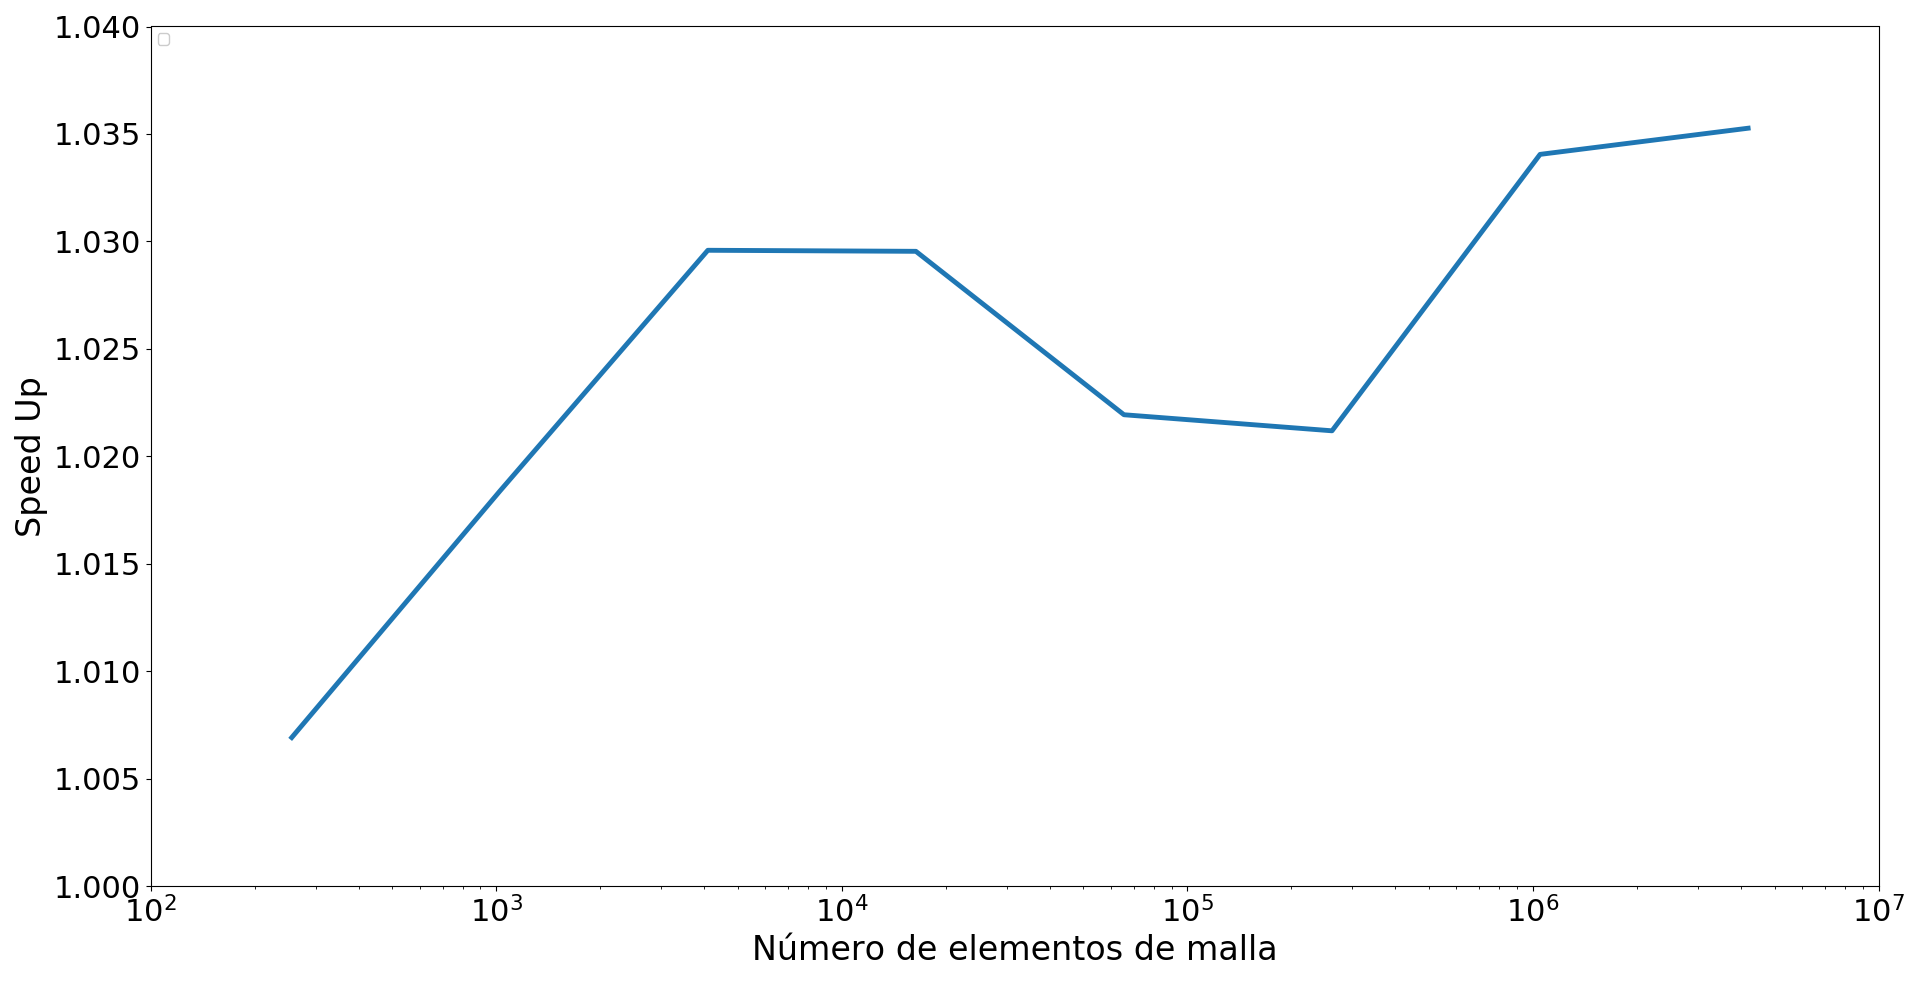
\includegraphics[width=\textwidth]{figs/cap4/c_970_MxC_c_10}
	\caption{Speed Up realizado para el problema de la Construcción de Maxwell con la GPU NVIDIA Geforce GTX 970 en en el código de \textbf{C}, comparando simple precisión y doble precisión.} 
	\label{fig:c_970_MxC_c_10}	
\end{figure}

\begin{figure}[h!]
	\centering
	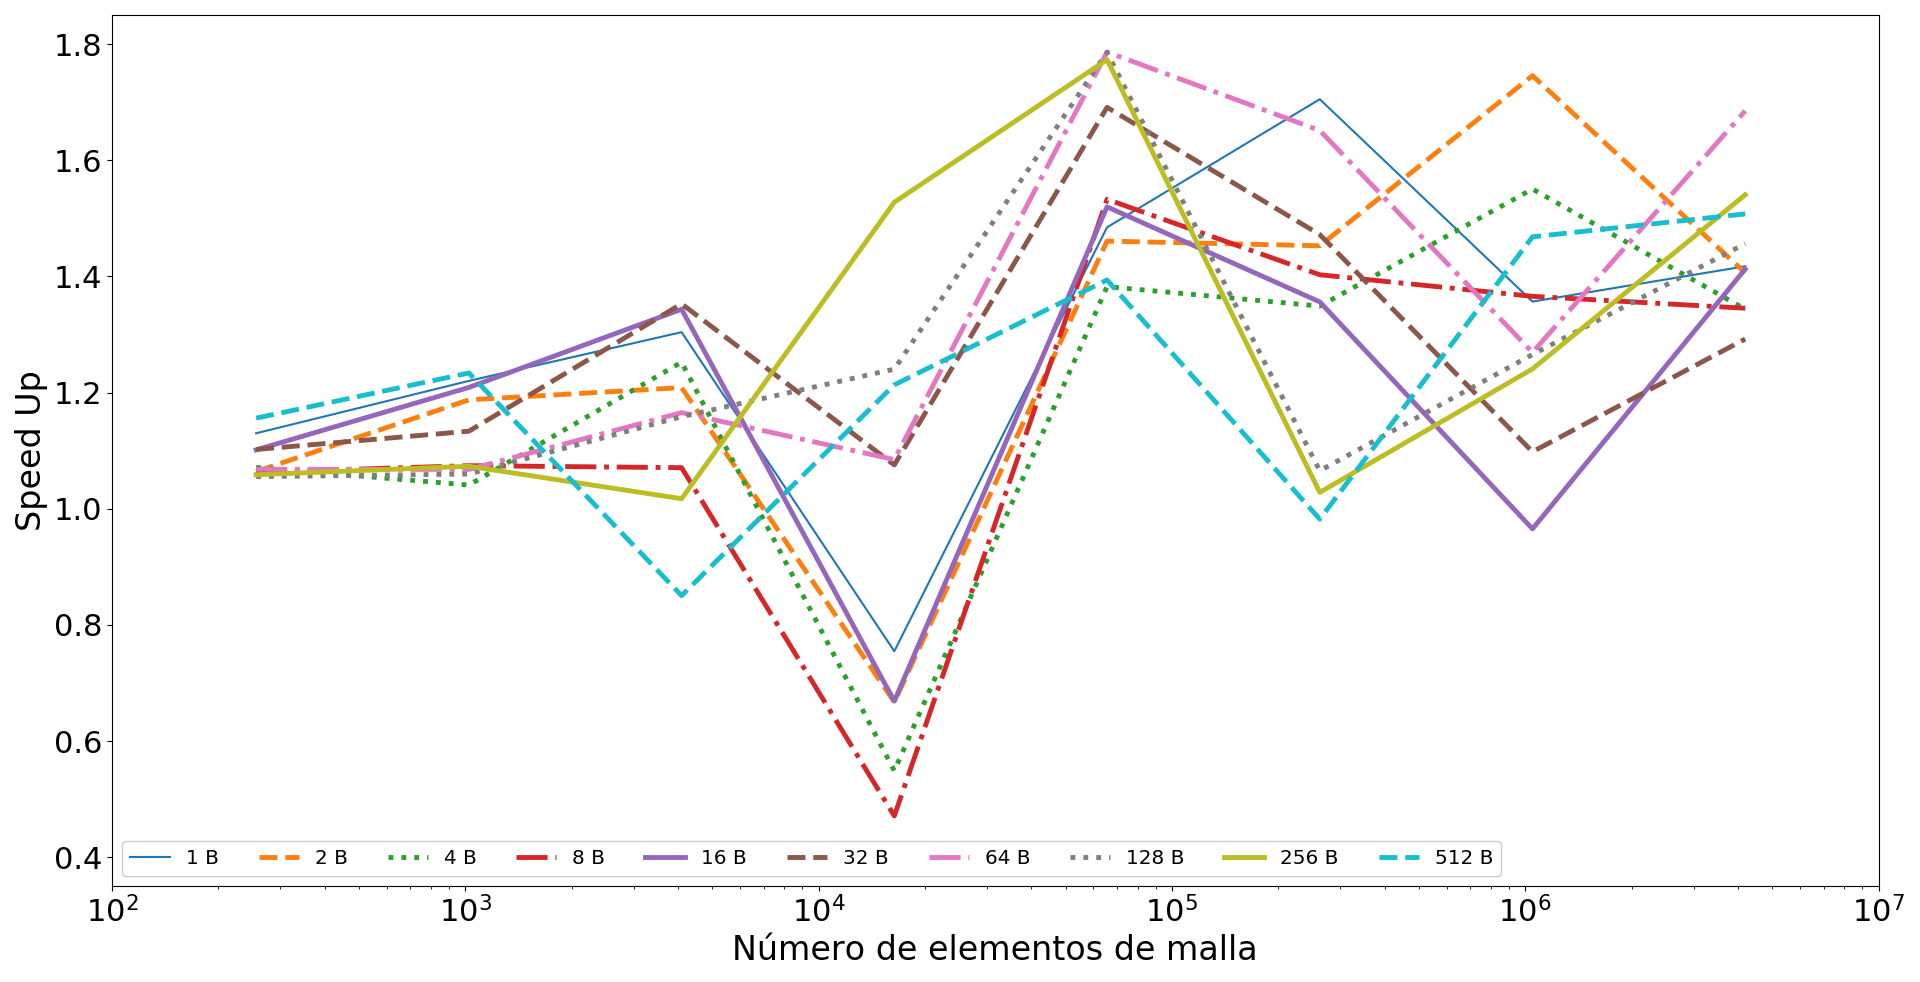
\includegraphics[width=\textwidth]{figs/cap4/c_970_MxC_cuda_10}
	\caption{Speed Up realizado para el problema de la Construcción de Maxwell con la GPU NVIDIA Geforce GTX 970 en en el código de \textbf{CUDA C}, comparando simple precisión y doble precisión.} 
	\label{fig:c_970_MxC_cuda_10}	
\end{figure}

Los valores que se obtuvieron en las Figuras (\ref{fig:s_970_MxC_simple_10}), (\ref{fig:s_970_MxC_double_10}), (\ref{fig:c_970_MxC_c_10}) y (\ref{fig:c_970_MxC_cuda_10}) se encuentran en el Apéndice \ref{apend_MxC_970}


\subsection{Análisis}

La utilización de simple precisión en el código de \textbf{CUDA C} es más conveniente que doble precisión. Una de las razones es que no hay demasiada diferencia entre los valores que se pueden obtener, según los resultados obtenidos no difirieren más del 0,003 \%. Otra de las razones es que debido a las mejoras obtenidas en los tiempos de cálculo en las placas NVIDIA Geforce GTX 760 y NVIDIA Geforce GTX 970 en el código de \textbf{CUDA C} de 18.67 y 23.39 respectivamente en simple precisión que el código de \textbf{C}. Las mejoras en doble precisión de las ganancias son de 11.40 y 10.96 respectivamente en las placas mencionadas. Por lo que el resultado obtenido en simple precisión difiere apenas un 0.003 \% que en doble precisión, además siendo 1.68 y 1.29 veces más rapido según la GPU utilizada.



\section{Estratificación de un fluido VdW con temperatura no uniforme}

Se quiere resolver el problema de tener una cavidad unidimensional en presencia de un fluido cuya EOS es la de Van der Waals; con temperatura  no uniforme y fuerza de gravedad no nula. Éste problema fue desarrollado por Berberan-Santos \cite{berberan2002liquid} y que Fogliatto \cite{fogliatto2019simulation} extendió. 

Se toma como coordenada del problema \textit{y}, teniéndose una temperatura fija $T_{0}$ en $y = 0$ y $T_{1}$ en $y = H$ como se observa en la Figura (xxxx) en presencia de la gravedad.

El gradiente de presión surge de realizar el balance de momento en un volumen de control, obteniéndose:

\begin{align}
	\frac{d P}{d y} = - g M C(y)
\end{align}

siendo \textit{g} la gravedad, \textit{M} el peso molecular, $C = \frac{1}{v}$ la fracción molar, \textit{v} el volumen molar y \textit{P} la presión.

Realizando la adimensionalisación de $ P_r = \frac{P}{P_c}$ , $ T_r = \frac{T}{T_c}$, $c = C v_c$ y $E_r = \frac{M g y}{R T_c}$; siendo \textit{c} el punto crítico en el cuál comienza la coexistencia de las dos fases, se pueden reemplazar en el gradiente de presión y una Ecuación de estado para obtener una ecuación adimensional con la concentración molar distribuida \cite{fogliatto2019simulation}.

Si se elije la EOS de VdW de la Ec.(\ref{eq:VdW_P}), se obtiene la siguiente ecuación adimensional diferencial:

\begin{align}
	\frac{d c}{d E_r} = - \left[ c + \frac{d T_r}{d E_r} \left( \frac{c}{1 - \frac{c}{3}}\right) \right] \left[	\frac{1}{\frac{T_r}{{\left(1- \frac{c}{3}\right)}^2} - \frac{9}{4} c}  \right] 
	\label{eq:adim_dif}
\end{align} 

Si se resuelve iterativamente la Ec. (\ref{eq:adim_dif}) se puede obtener dos curvas adimensionales correspondientes al perfil de temperatura y al de concentraciones.

En la Figura xx se muestra la curva adimensional $ \rho_r - Y_r $ , siendo $\rho_r = \frac{\rho}{\rho_c}$ y  $Y_r = \frac{y}{H}$  y la Figura xx muestra la curva adimensional $ T_r - Y_r $. Ambas para distintos valores de $T_0$, mientras que en la otra pared $T_1 = cte = 0.99 \> T_r$.

\begin{figure}[h!]
	\centering
	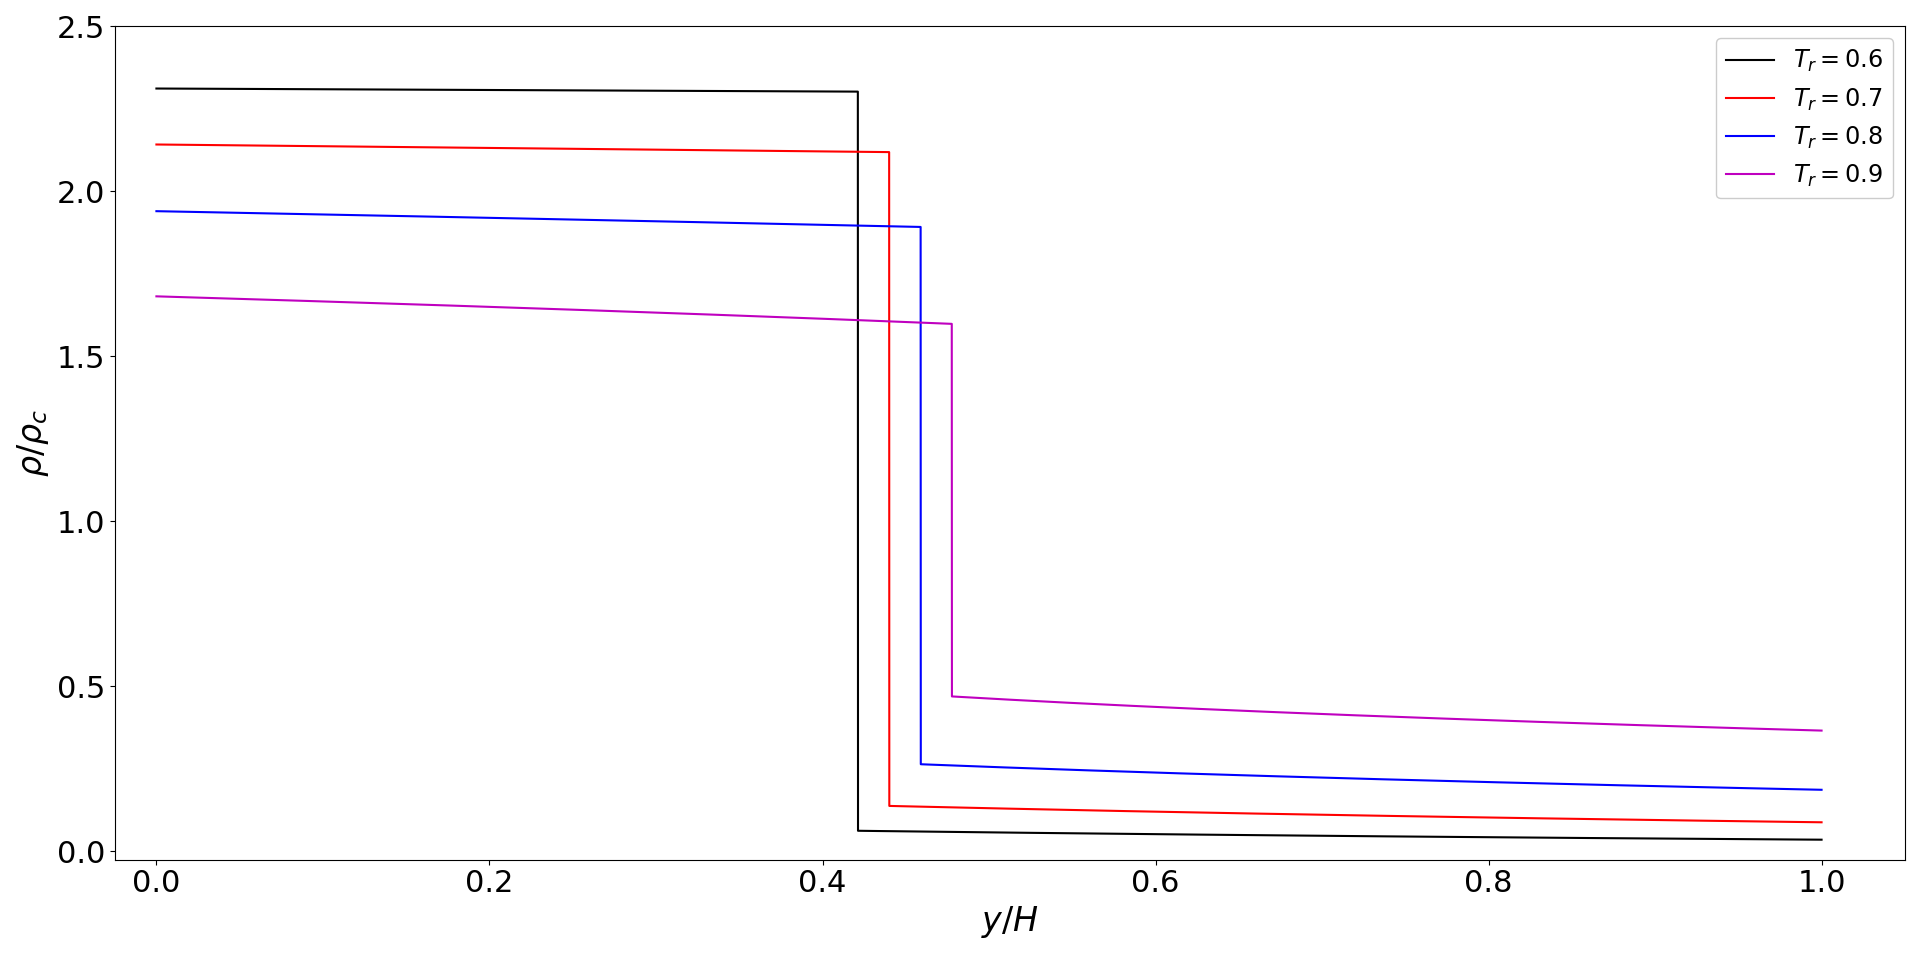
\includegraphics[width=\textwidth]{figs/cap4/VdW_val_rho_y}
	\caption{Perfil de densidad adimensional a lo largo de la longitud de la pared,para distintos valores de condición de temperatura fija en $y = 0$, para un fluido de VdW con los parámetros $a = 0,5 $ y $b = 4,0 $, obtenida en simple precisión en la GPU NVIDIA Geforce GTX 760 en el código desarrollado en \textbf{C}.} 
	\label{fig:VdW_val_rho_y}	
\end{figure}

\begin{figure}[h!]
	\centering
	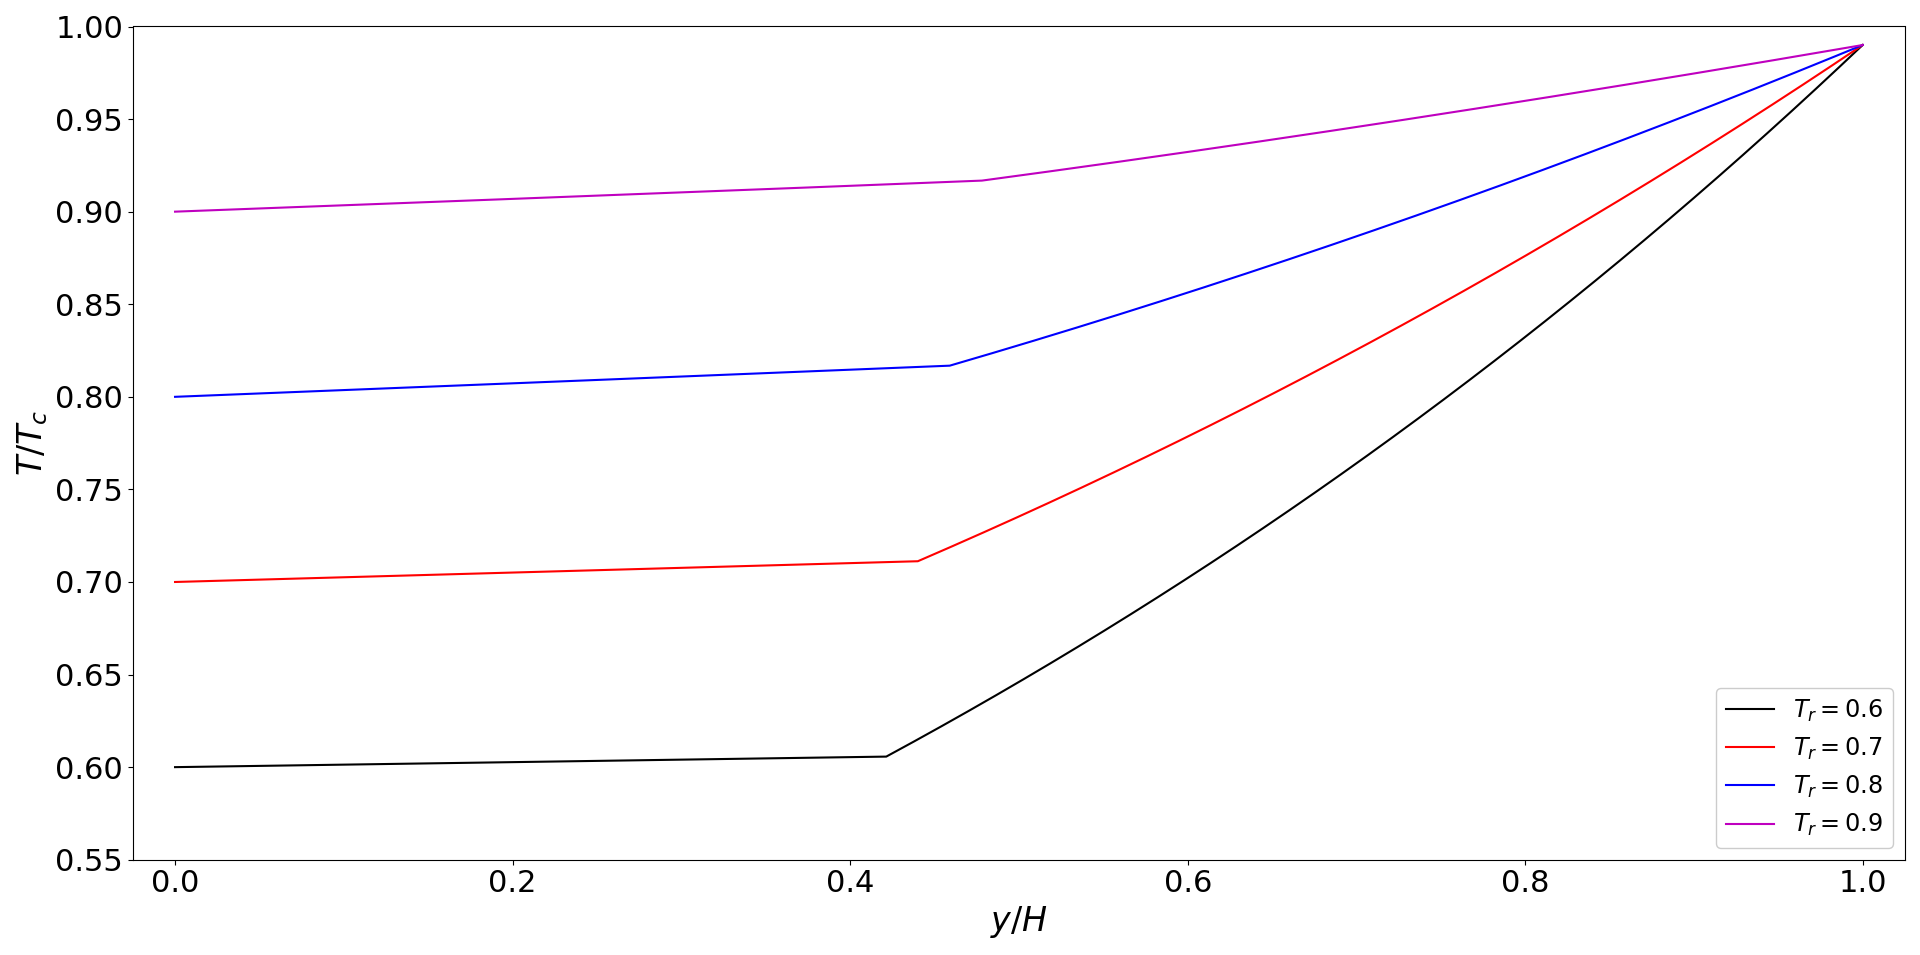
\includegraphics[width=\textwidth]{figs/cap4/VdW_val_T_y}
	\caption{Perfil de temperatura adimensional a lo largo de la longitud de la pared, para distintos valores de condición de temperatura fija en $y = 0$,para un fluido de VdW con los parámetros $a = 0,5 $ y $b = 4,0 $, obtenida en simple precisión en la GPU NVIDIA Geforce GTX 760 en el código desarrollado en \textbf{C}.} 
	\label{fig:VdW_val_T_y}	
\end{figure}

\newpage

\subsection{Validación}

La validación de éste problema se hizo utilizando los parámetros $a =0,5$ y $b = 4,0$; para un tamaño de malla de 3 x 300 nodos y $T_0 = T_r$, variando $T_r$ con un paso de $0,025$ en el rango de $[0,6 - 0,975]$. Mostrándose en los gráficos únicamente los valores de $T_r = 0,6 ; 0,7 ; 0,8 y 0,9$   El valor de $\mathbf{M}$ utilizado es el mismo que es de la Construcción de Maxwell, mientras que el valor de $\Lambda$ se encuentran en el Apéndice (xxxx).

La Figura(\ref{fig:v_760_VdW_c_simple_rho_y}) y (\ref{fig:v_760_VdW_c_simple_T_y})  muestran la validación del código realizado en \textbf{C} para simple precisión en una GPU NVIDIA Geforce GTX 760; con distintos valores de $T_0$. 

El quiebre abrupto y discontínuo de la densidad a lo largo de la pared en la Figura (\ref{fig:v_760_VdW_c_simple_rho_y}) muestra la coexistencia de las dos fases, para la solución analítica. Debido a que se tiene una solución contínua y un poco difusa porque el modelo toma una cierta cantidad de nodos como separación entre ambas fases, se presenta una mayor diferencia en el ajuste de la curva obtenida con la analítica en el cambio de fase. Lo mismo sucede en la Figura (\ref{fig:v_760_VdW_c_simple_T_y}).

El tiempo de vuelo utilizado en cada uno de los nodos de la malla fue de 750000. 
El resultado obtenido para ambas curvas validades es exactamente igual en el código de \textbf{C} y \textbf{CUDA C}.

\begin{figure}[h!]
	\centering
	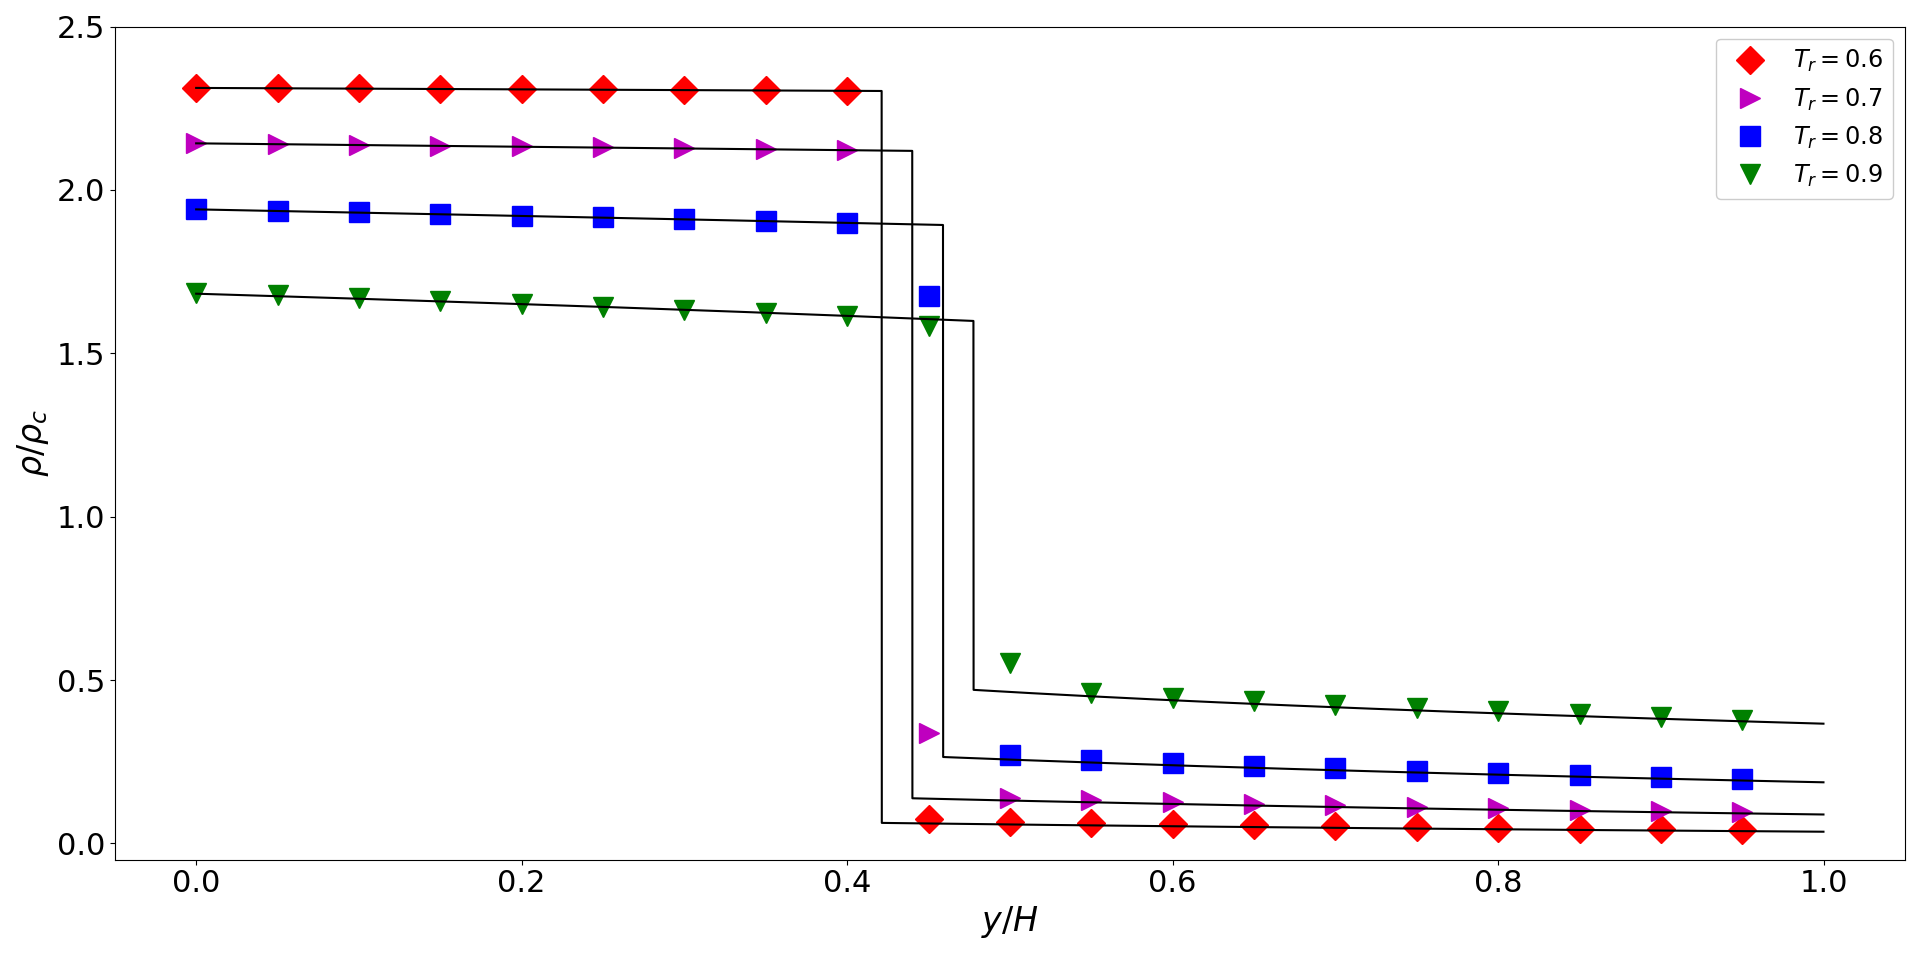
\includegraphics[width=\textwidth]{figs/cap4/v_760_VdW_c_simple_rho_y}
	\caption{Perfil de densidad adimensional a lo largo de la longitud de la pared, para valores de $T_0 = T_r$ , siendo $T_r = 0,6 ; 0,7 ; 0,8 y 0,9$, para un fluido de VdW con los parámetros $a = 0,5 $ y $b = 4,0 $, obtenida en simple precisión en la GPU NVIDIA Geforce GTX 760 en el código desarrollado en \textbf{C}.}
	\label{fig:v_760_VdW_c_simple_rho_y}	
\end{figure}

\begin{figure}[h!]
	\centering
	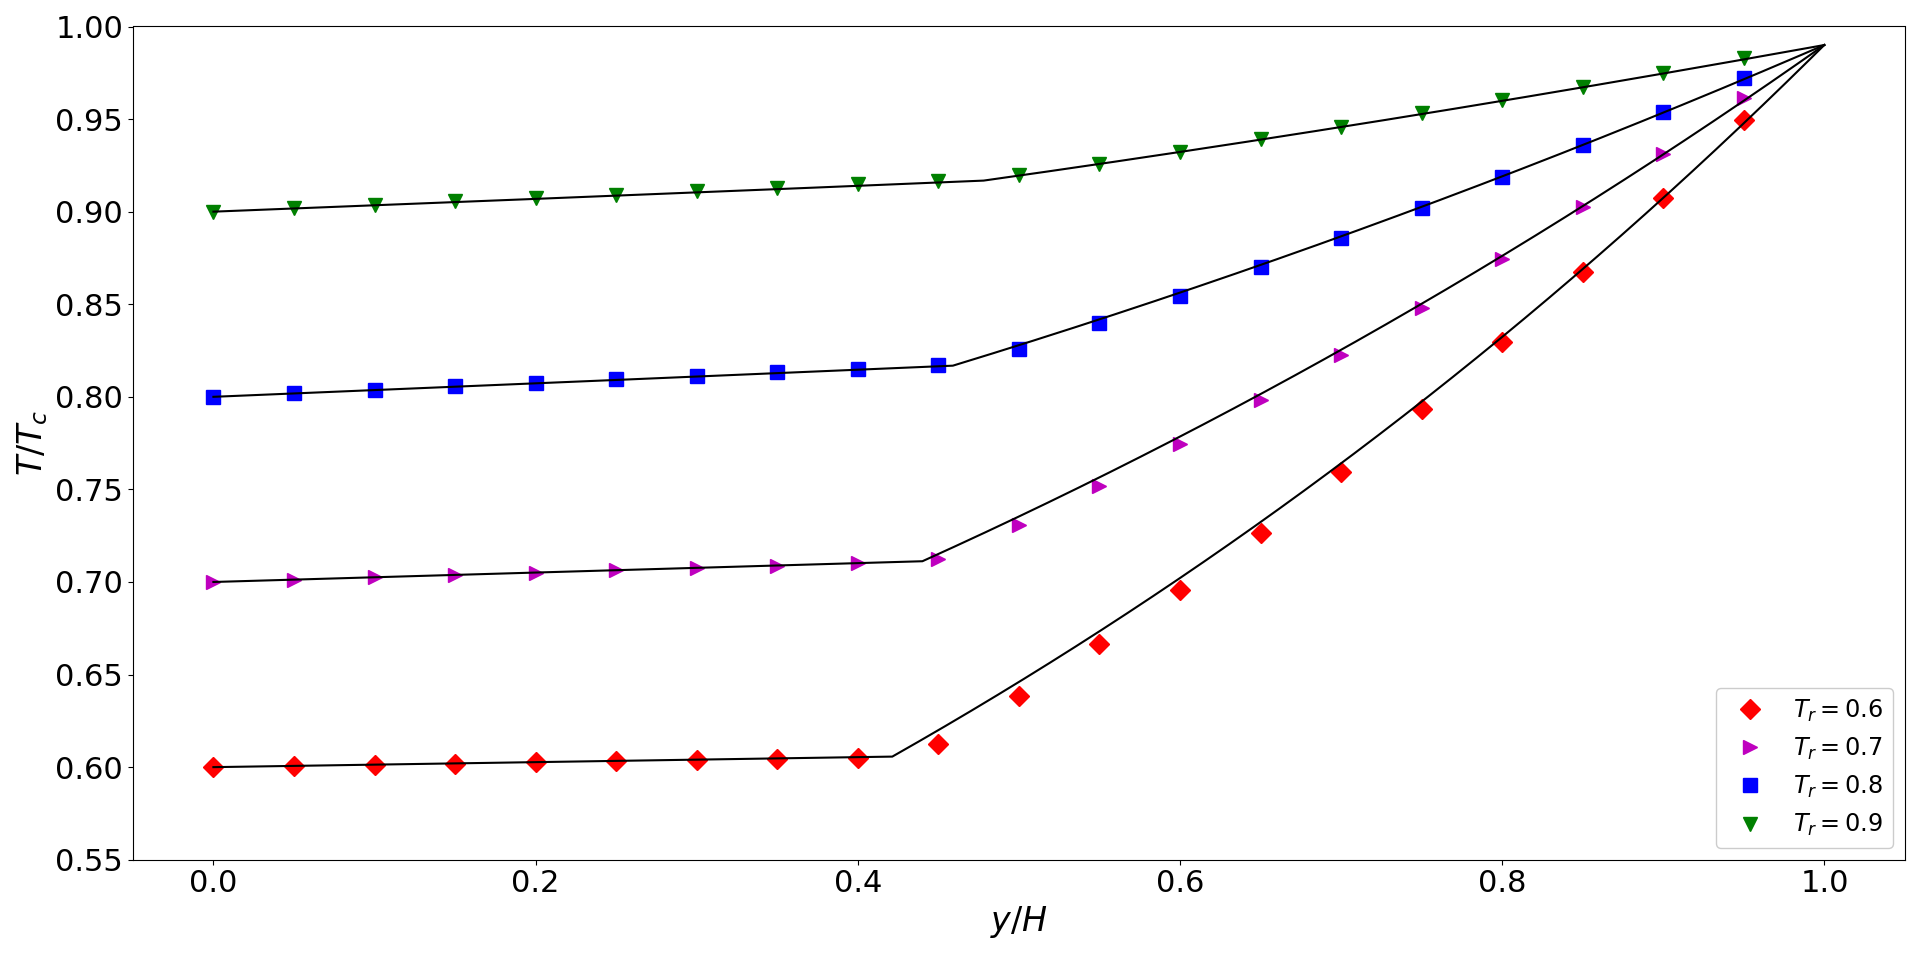
\includegraphics[width=\textwidth]{figs/cap4/v_760_VdW_c_simple_T_y}
	\caption{Perfil de temperatura adimensional a lo largo de la longitud de la pared, para valores de $T_0 = T_r$ , siendo $T_r = 0,6 ; 0,7 ; 0,8 \>y\> 0,9$, para un fluido de VdW con los parámetros $a = 0,5 $ y $b = 4,0 $, obtenida en simple precisión en la GPU NVIDIA Geforce GTX 760 en el código desarrollado en \textbf{C}.}
	\label{fig:v_760_VdW_c_simple_T_y}	
\end{figure}

\newpage

\subsection{Speed Up}

En la presente sección se muestran las mejora en el tiempo de cálculo realizados para el código de \textbf{C} y \textbf{CUDA C}. La comparación se realizó en simple y doble precisión; en las GPU NVIDIA Geforce GTX 760 y NVIDIA Geforce GTX 970. Se tomó una $T_r$ fija y se varió el tamaño de la grilla, de manera que ésta siempre tuviese un ancho constante de 300 nodos y variando la dimensión en el eje \textsc{Y} respetando un número de nodos de potencia de 2 (exceptuando el primer valor que es 3) . La cantidad de \textit{thread blocks} que se utilizó para realizar la comnparación en el código de \textbf{CUDA} fueron de potencia de 2.

\subsubsection{NVIDIA Geforce GTX 760}

Los tamaños de grilla que se utilizaron para realizar las pruebas de tiempo de ésta placa, tienen el rango de grilla de 3x300 nodos hasta 1638400x300 nodos. La cantidad de \textit{thread blocks} que se utilizó fueron de 1 a 512.

Las Figuras (\ref{fig:s_760_VdW_simple_10}) y (\ref{fig:s_760_VdW_double_10}) muestran el \textit{Speed Up} obtenido comparando los códigos de \textbf{C} y \textbf{CUDA C}, donde la Figura (\ref{fig:s_760_VdW_simple_10}) está obtenida con simple precisión y la Figura (\ref{fig:s_760_VdW_double_10}) en doble precisión. El mejor resultado en ambos casos se obtuvo para un número de \textit{thread block} igual a 64, donde la mejora fue de 13.26 y 7.88 en simple y doble precisión respectivamente, para el mayor número de elementos de malla.


\begin{figure}[h!]
	\centering
	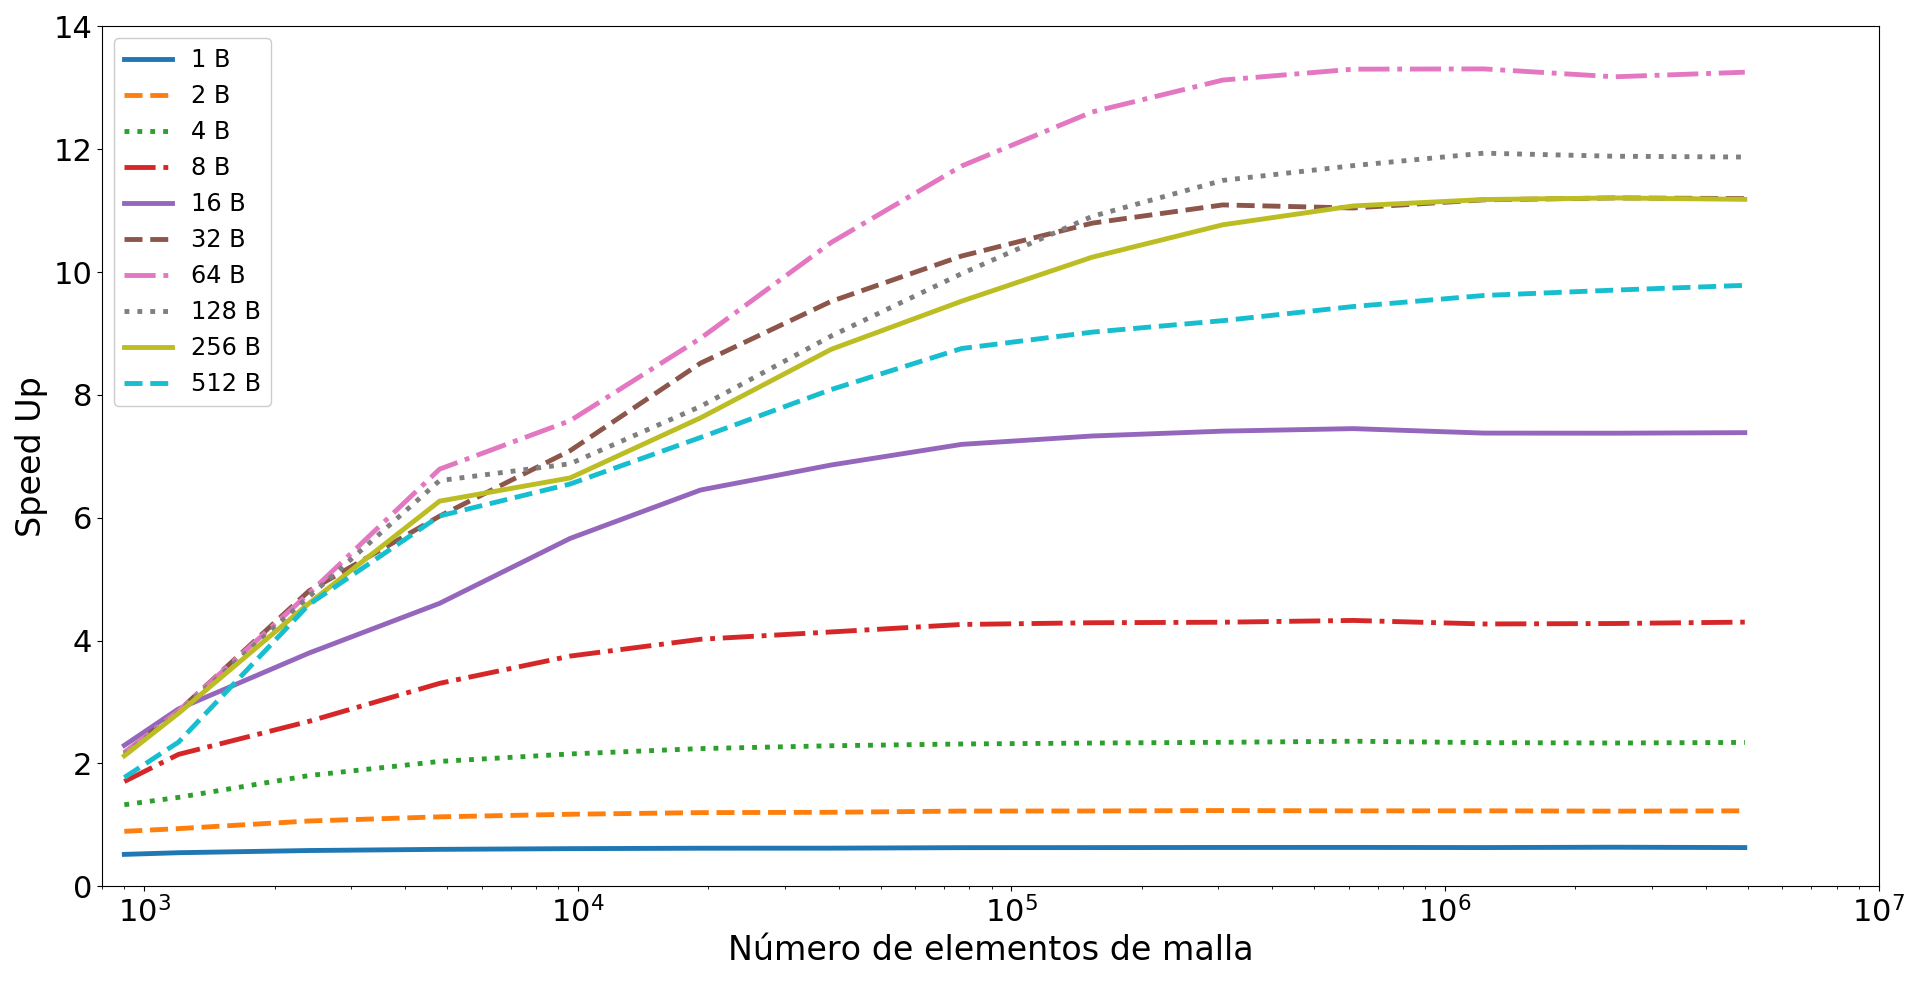
\includegraphics[width=\textwidth]{figs/cap4/s_760_VdW_simple_10}
	\caption{Speed Up realizado para el problema de la Estratificación de un fluido Van der Waals con la GPU NVIDIA Geforce GTX 760 en simple precisión, comparando los códigos de \textbf{C} y \textbf{CUDA C}.} 
	\label{fig:s_760_VdW_simple_10}	
\end{figure}

\begin{figure}[h!]
	\centering
	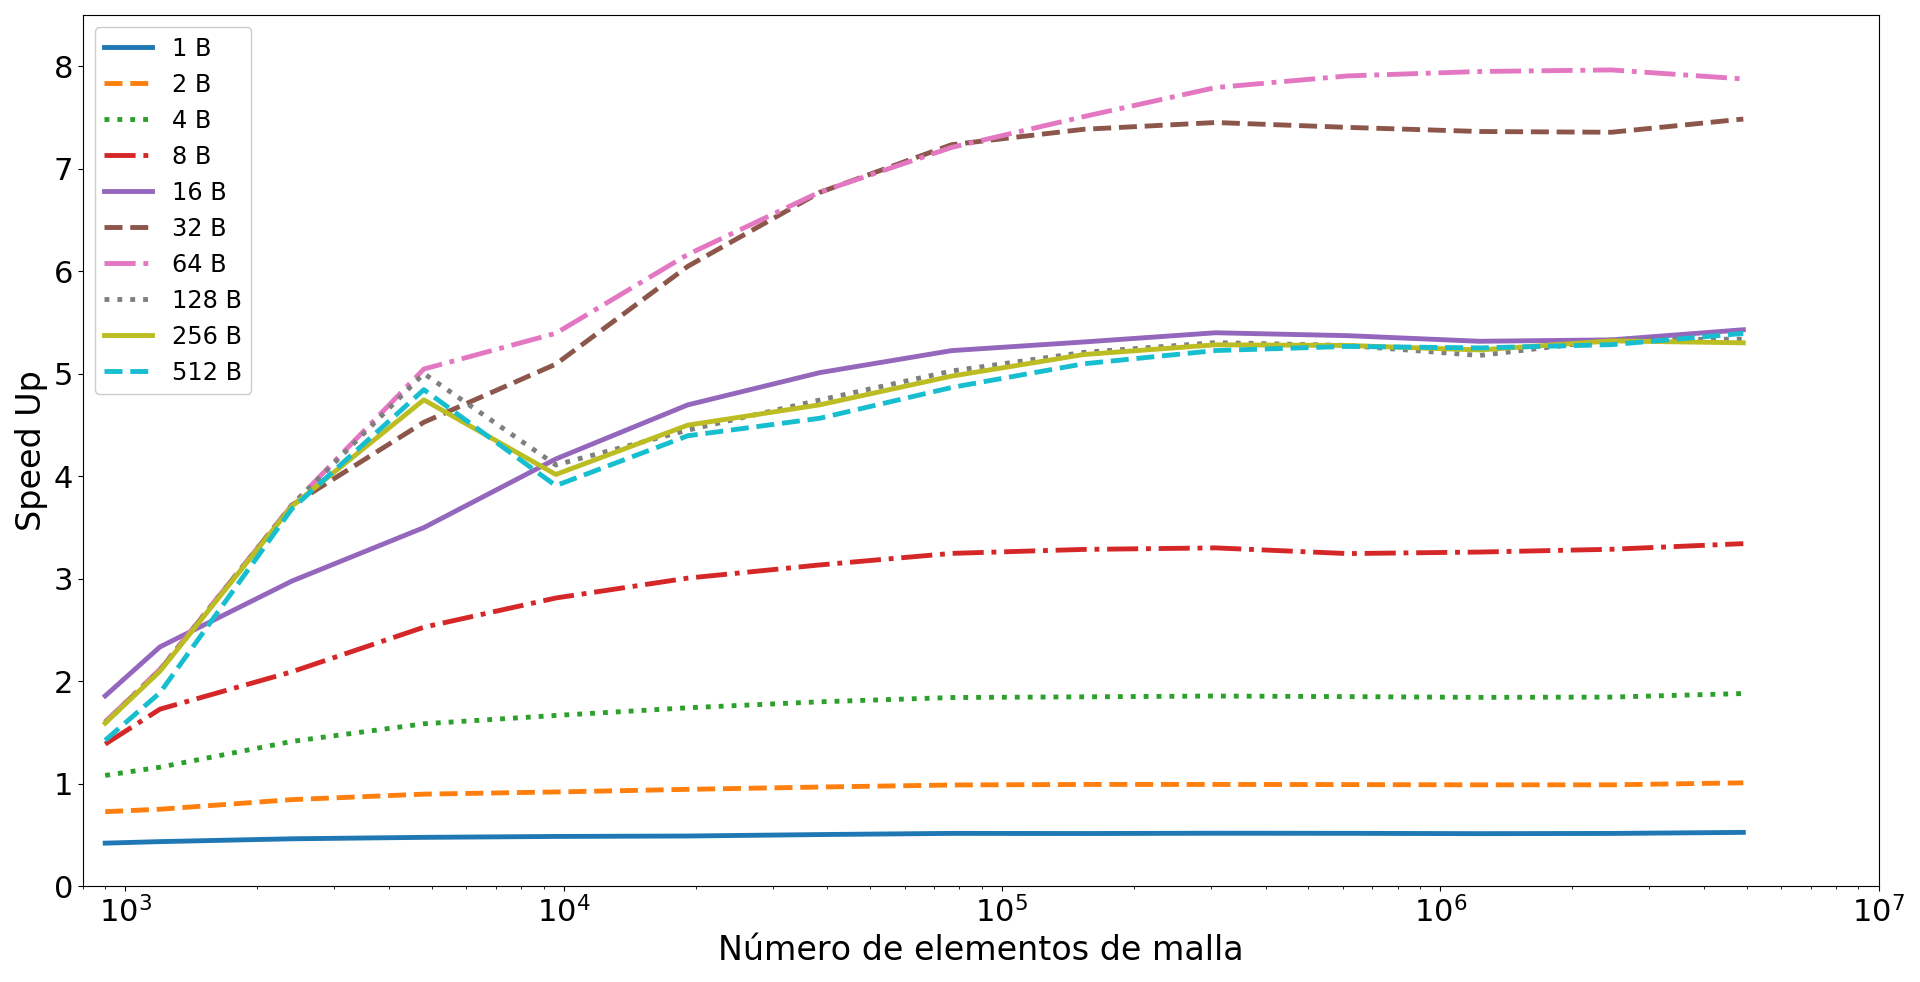
\includegraphics[width=\textwidth]{figs/cap4/s_760_VdW_double_10}
	\caption{Speed Up realizado para el problema de la Estratificación de un fluido Van der Waals con la GPU NVIDIA Geforce GTX 760 en doble precisión, comparando los códigos de \textbf{C} y \textbf{CUDA C}.} 
	\label{fig:s_760_VdW_double_10}	
\end{figure}

\newpage

Las Figuras (\ref{fig:c_760_VdW_c_10}) y (\ref{fig:c_760_VdW_cuda_10}) muestran el \textit{Speed Up} obtenido comparando simple precisión y doble precisión, donde la Figura (\ref{fig:c_760_VdW_c_10}) está obtenida el código de \textbf{C} y la Figura (\ref{fig:c_760_VdW_cuda_10}) en el código de \textbf{CUDA C}. 

En el código de \textbf{C} para el mayor número de elementos de la malla, el resultado de tiempos de cálculo en doble precisión es apenas 1,052 veces mayor que en  simple precisión. En contraste, al fijarse el resultado para un número de \textit{thread block} igual a 64 (el que mayor ganancia obtuvo), el tiempo de cálculo en doble precisión es 1,77 veces mayor que en simple precisión; para el mayor número de elementos de malla calculado.

\begin{figure}[h!]
	\centering
	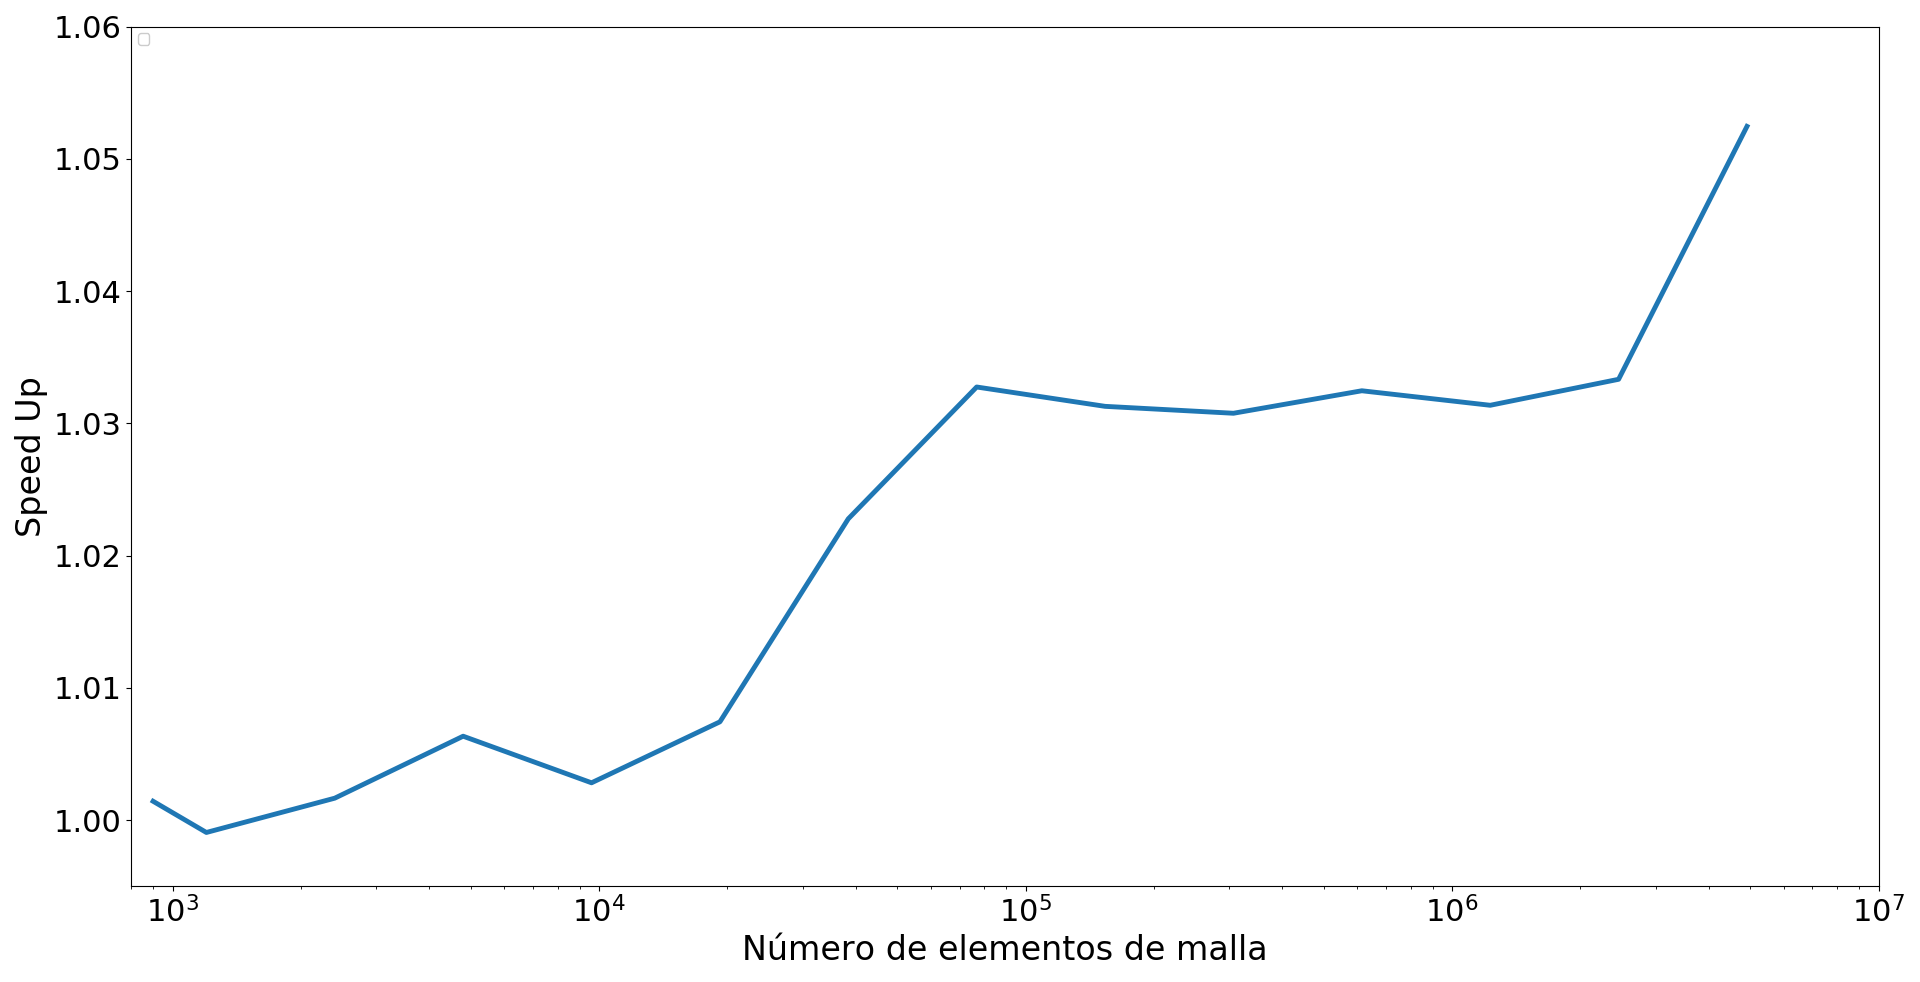
\includegraphics[width=\textwidth]{figs/cap4/c_760_VdW_c_10}
	\caption{Speed Up realizado para el problema de la Estratificación de un fluido Van der Waals con la GPU NVIDIA Geforce GTX 760 en en el código de \textbf{C}, comparando simple precisión y doble precisión.} 
	\label{fig:c_760_VdW_c_10}	
\end{figure}

\begin{figure}[h!]
	\centering
	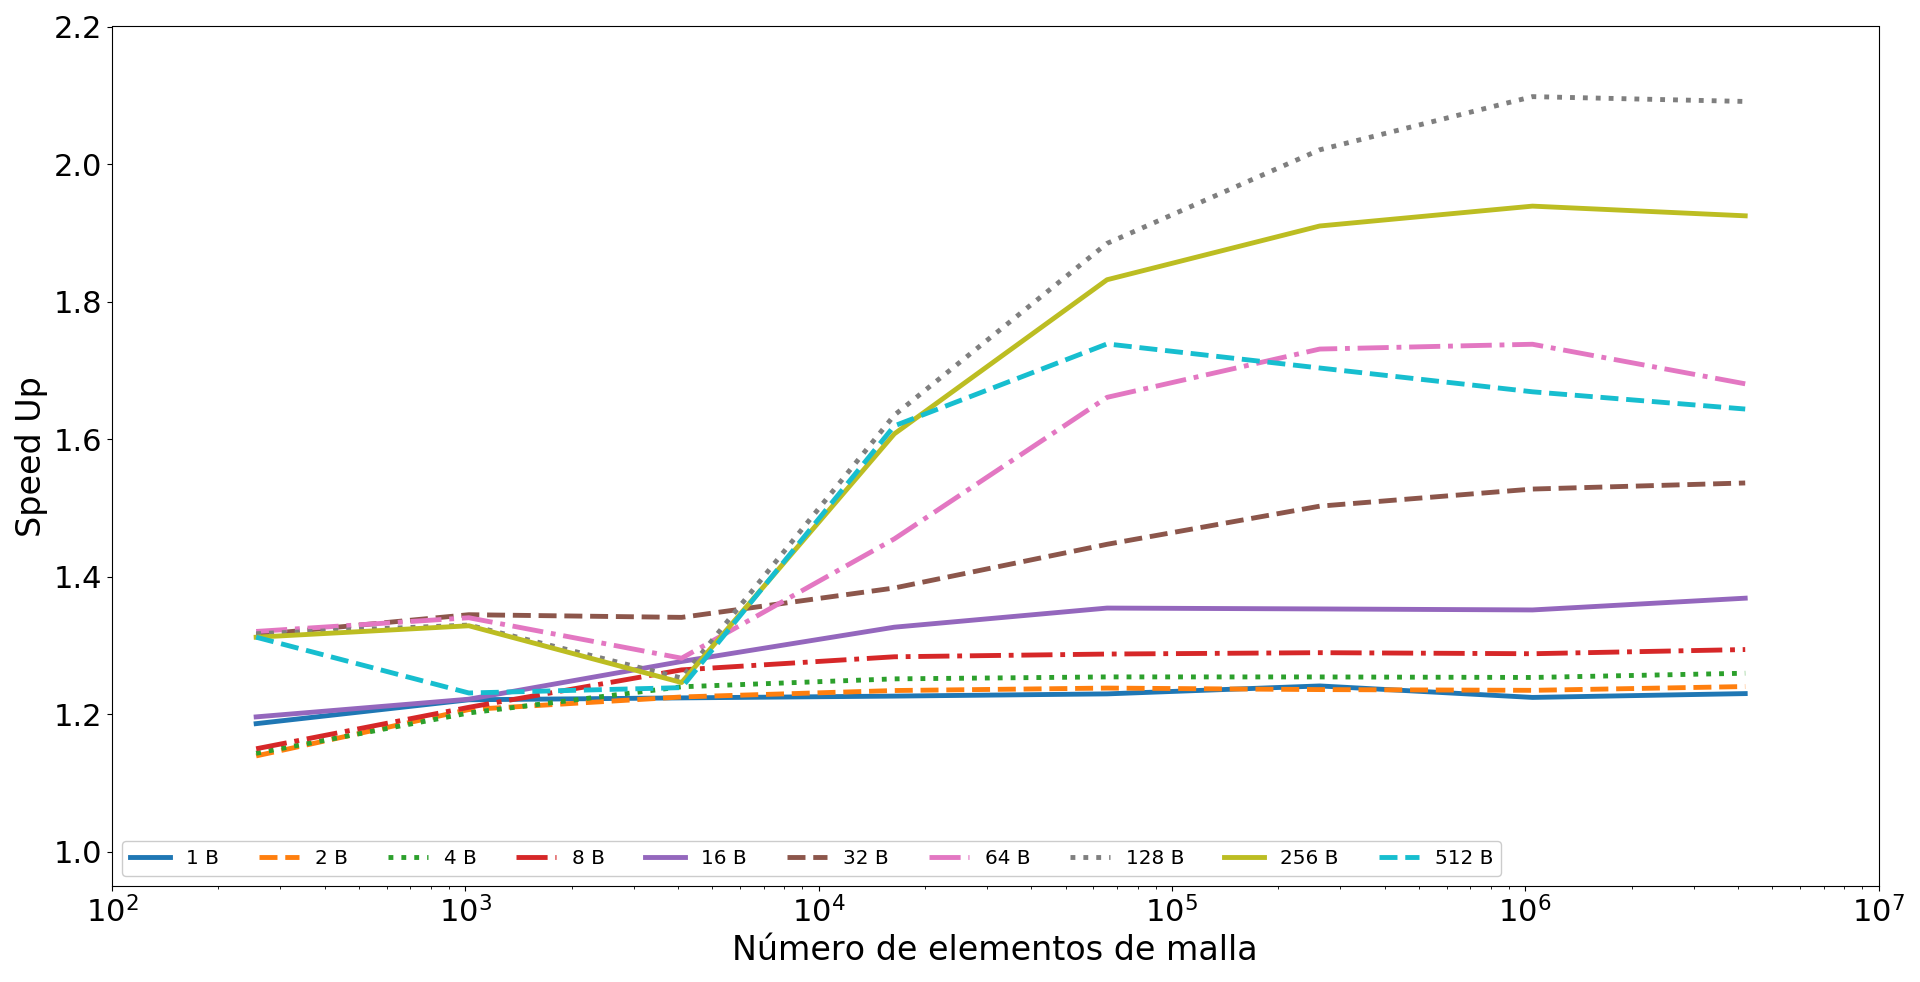
\includegraphics[width=\textwidth]{figs/cap4/c_760_MxC_cuda_10}
	\caption{Speed Up realizado para el problema de la Estratificación de un fluido Van der Waals con la GPU NVIDIA Geforce GTX 760 en en el código de \textbf{CUDA C}, comparando simple precisión y doble precisión.} 
	\label{fig:c_760_VdW_cuda_10}	
\end{figure}

Los valores que se obtuvieron en las Figuras (\ref{fig:s_760_VdW_simple_10}), (\ref{fig:s_760_VdW_double_10}), (\ref{fig:c_760_VdW_c_10}) y (\ref{fig:c_760_VdW_cuda_10}) se encuentran en el Apéndice \ref{apend_VdW_760}

\newpage

\subsubsection{NVIDIA Geforce GTX 970}

Los tamaños de grilla que se utilizaron para realizar las pruebas de tiempo de ésta placa, tienen el rango de grilla de 3x300 nodos hasta 1638400x300 nodos. La cantidad de \textit{thread blocks} que se utilizó fueron de 1 a 512.

Las Figuras (\ref{fig:s_970_VdW_simple_10}) y (\ref{fig:s_970_VdW_double_10}) muestran el \textit{Speed Up} obtenido comparando los códigos de \textbf{C} y \textbf{CUDA C}, donde la Figura (\ref{fig:s_970_VdW_simple_10}) está obtenida con simple precisión y la Figura (\ref{fig:s_970_VdW_double_10}) en doble precisión. El mejor resultado en ambos casos se obtuvo para un número de \textit{thread block} igual a 32, donde la mejora fue de 15.95 y 13.29 en simple y doble precisión respectivamente, para el mayor número de elementos de malla.


\begin{figure}[h!]
	\centering
	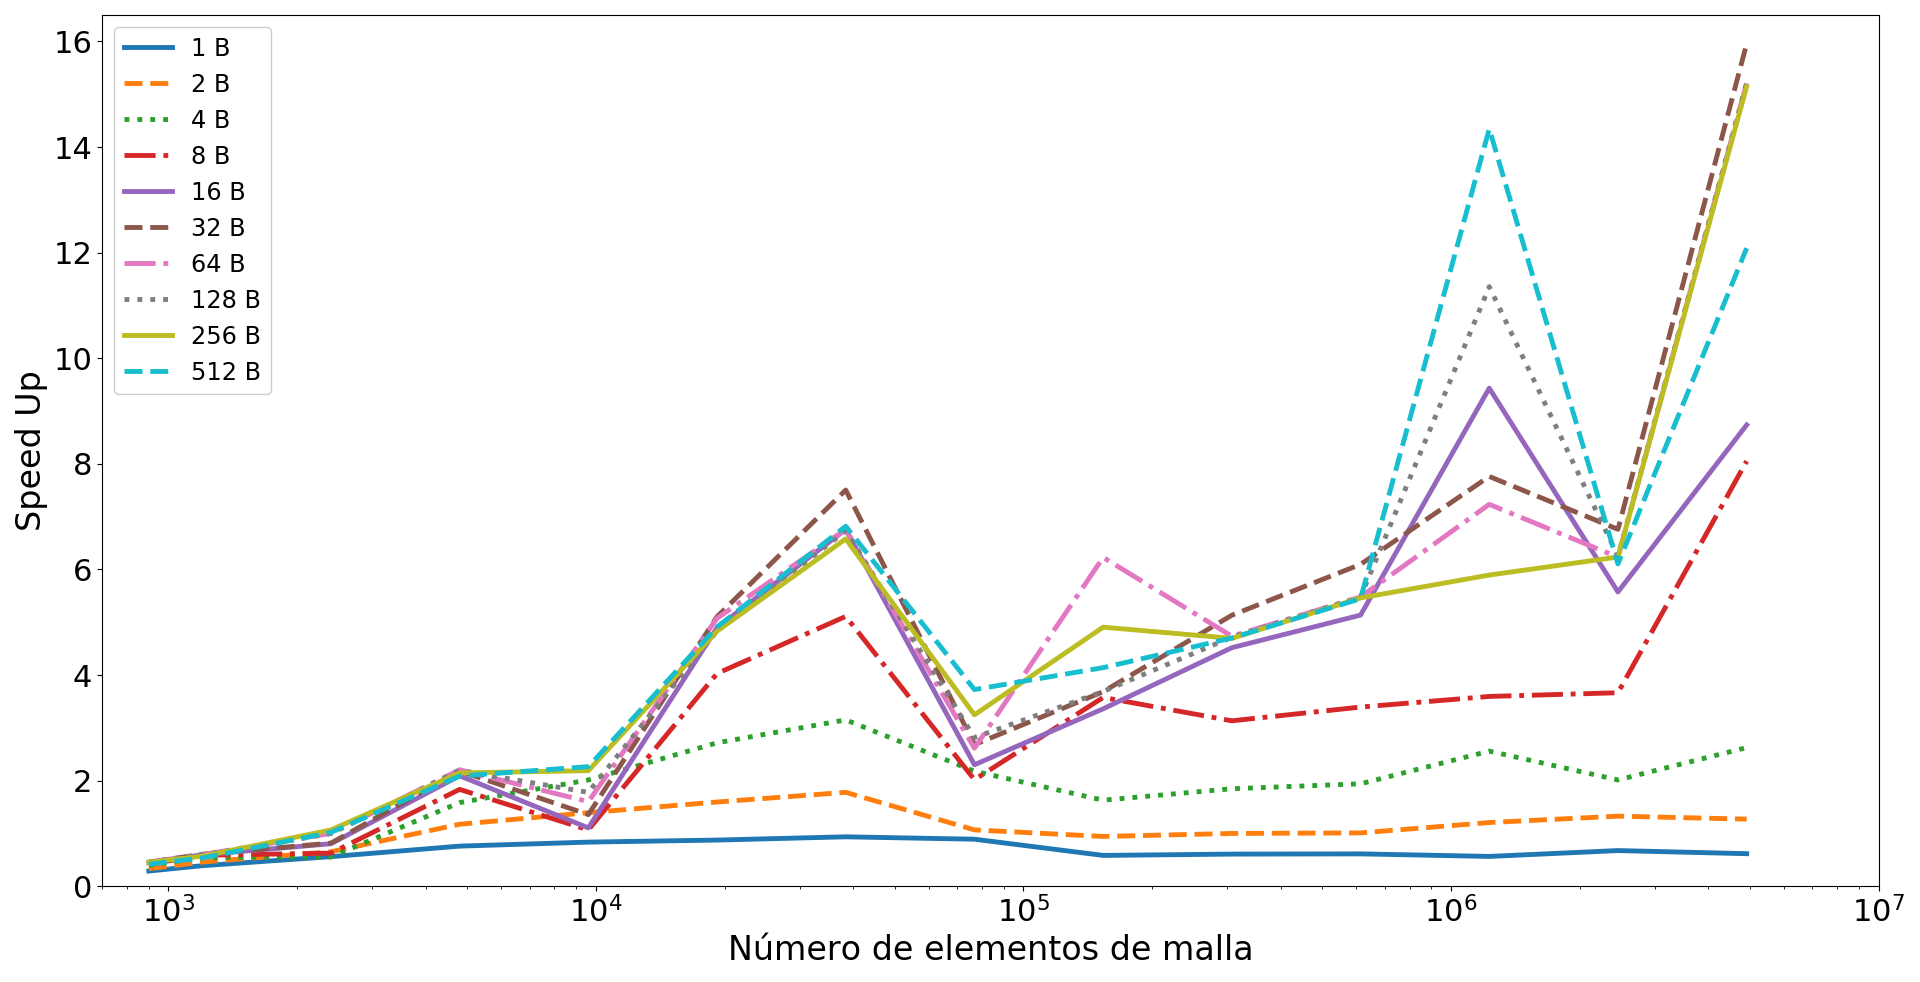
\includegraphics[width=\textwidth]{figs/cap4/s_970_VdW_simple_10}
	\caption{Speed Up realizado para el problema de la Estratificación de un fluido Van der Waals con la GPU NVIDIA Geforce GTX 970 en simple precisión, comparando los códigos de \textbf{C} y \textbf{CUDA C}.} 
	\label{fig:s_970_VdW_simple_10}	
\end{figure}

\begin{figure}[h!]
	\centering
	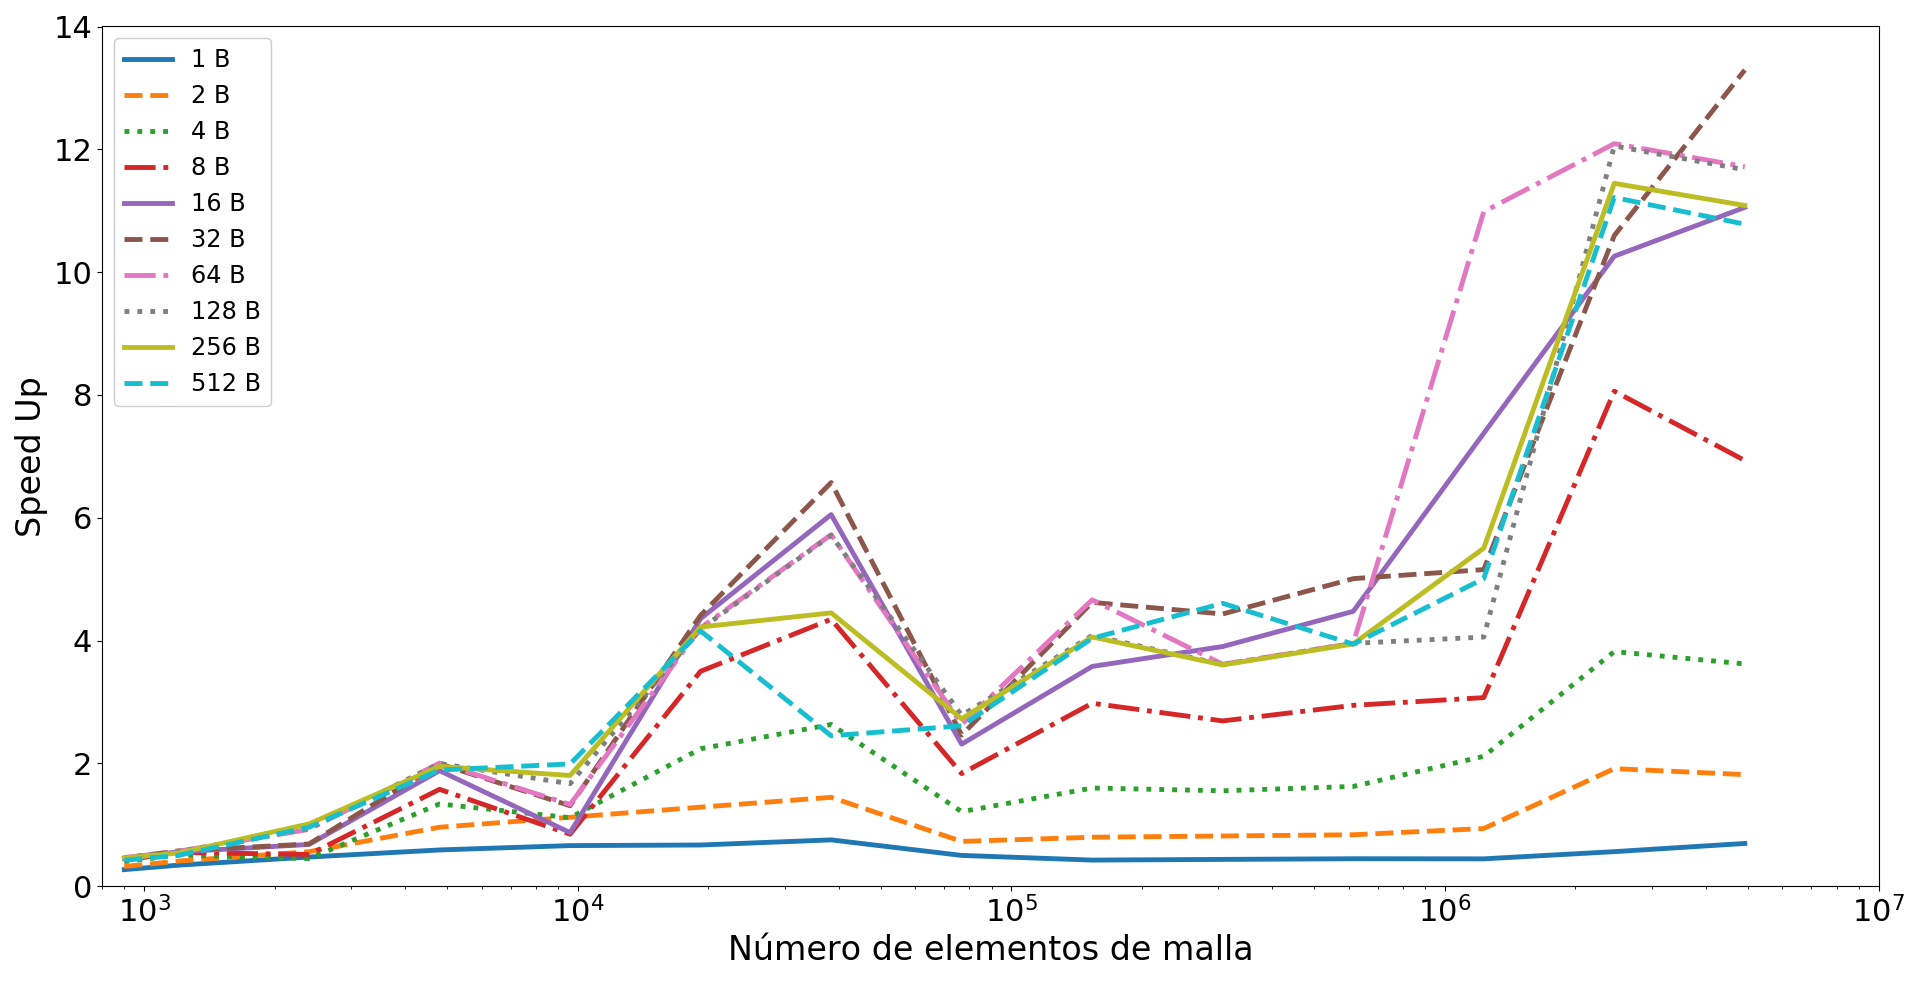
\includegraphics[width=\textwidth]{figs/cap4/s_970_VdW_double_10}
	\caption{Speed Up realizado para el problema de la Estratificación de un fluido Van der Waals con la GPU NVIDIA Geforce GTX 970 en doble precisión, comparando los códigos de \textbf{C} y \textbf{CUDA C}.} 
	\label{fig:s_970_VdW_double_10}	
\end{figure}

\newpage

Las Figuras (\ref{fig:c_970_VdW_c_10}) y (\ref{fig:c_970_VdW_cuda_10}) muestran el \textit{Speed Up} obtenido comparando simple precisión y doble precisión, donde la Figura (\ref{fig:c_970_VdW_c_10}) está obtenida el código de \textbf{C} y la Figura (\ref{fig:c_970_VdW_cuda_10}) en el código de \textbf{CUDA C}. 

En el código de \textbf{C} para el mayor número de elementos de la malla, el resultado de tiempos de cálculo en doble precisión es apenas 1,045 veces mayor que en  simple precisión. En contraste, al fijarse el resultado para un número de \textit{thread block} igual a 32 (el que mayor ganancia obtuvo), el tiempo de cálculo en doble precisión es 1,25 veces mayor que en simple precisión; para el mayor número de elementos de malla calculado.

\begin{figure}[h!]
	\centering
	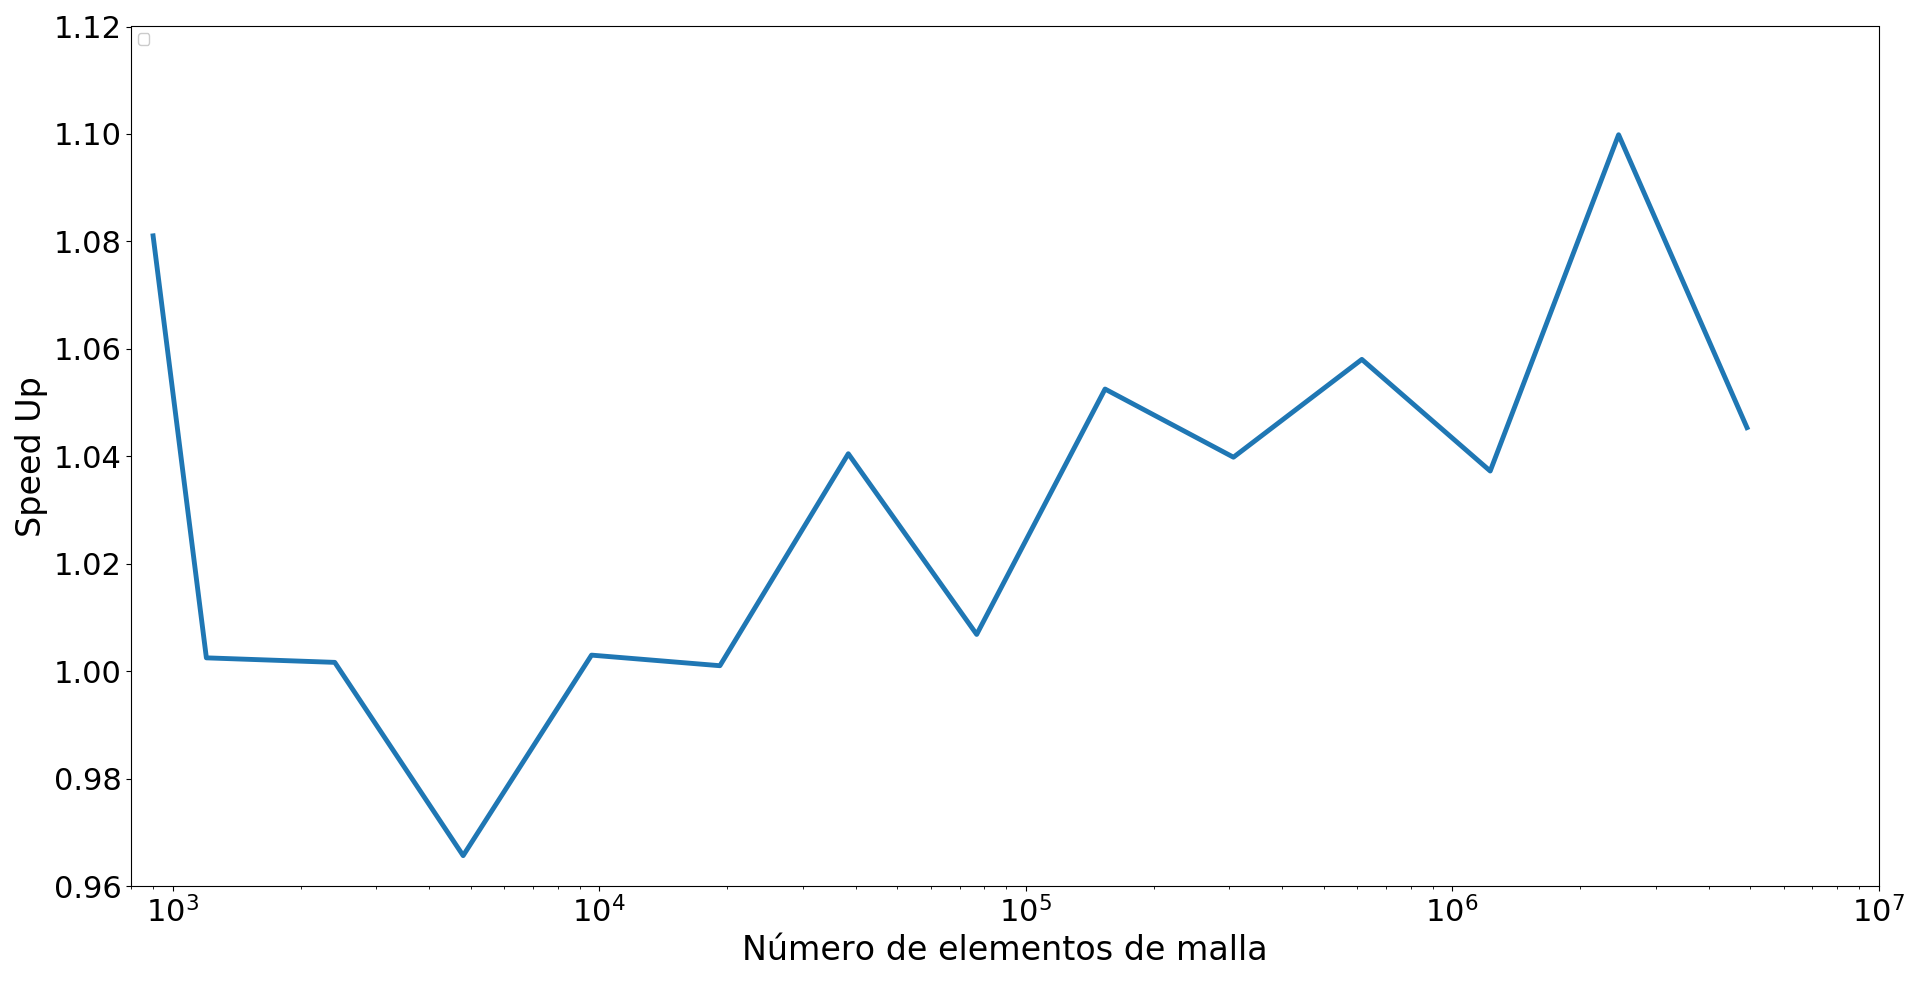
\includegraphics[width=\textwidth]{figs/cap4/c_970_VdW_c_10}
	\caption{Speed Up realizado para el problema de la Estratificación de un fluido Van der Waals con la GPU NVIDIA Geforce GTX 970 en en el código de \textbf{C}, comparando simple precisión y doble precisión.} 
	\label{fig:c_970_VdW_c_10}	
\end{figure}

\begin{figure}[h!]
	\centering
	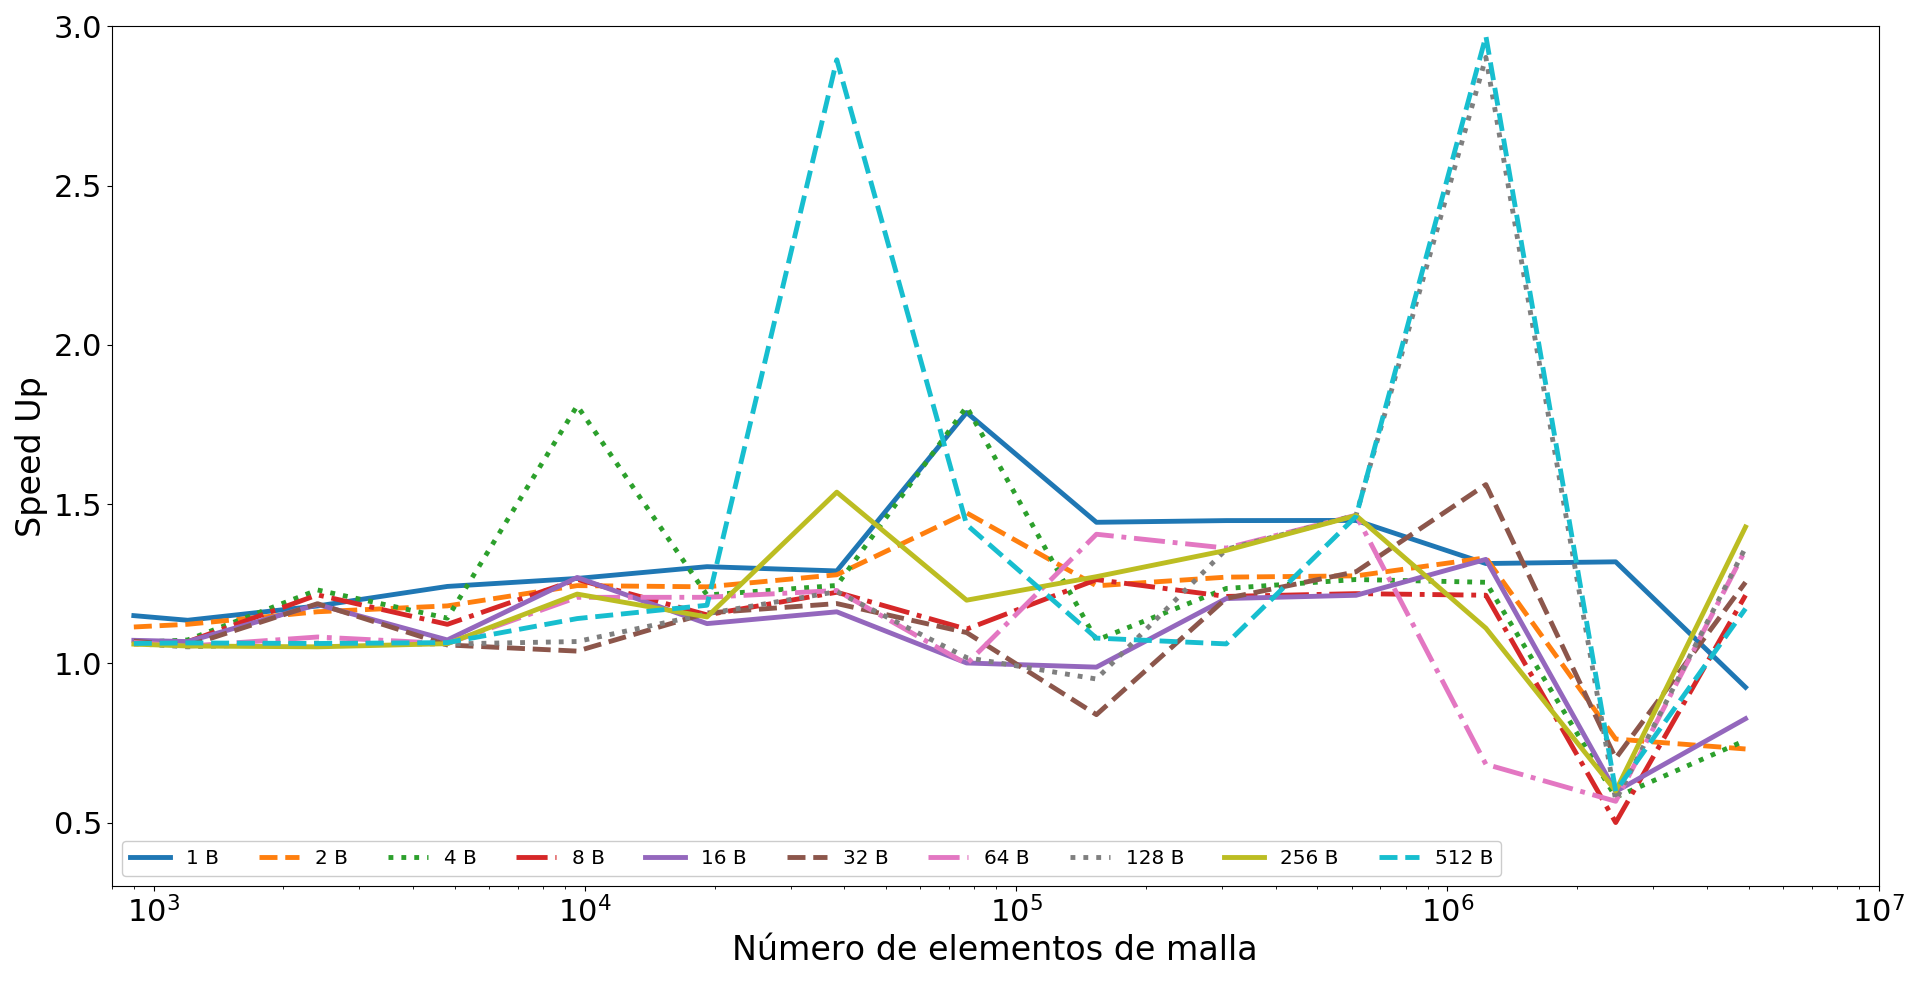
\includegraphics[width=\textwidth]{figs/cap4/c_970_VdW_cuda_10}
	\caption{Speed Up realizado para el problema de la Estratificación de un fluido Van der Waals con la GPU NVIDIA Geforce GTX 970 en en el código de \textbf{CUDA C}, comparando simple precisión y doble precisión.} 
	\label{fig:c_970_VdW_cuda_10}	
\end{figure}

Los valores que se obtuvieron en las Figuras (\ref{fig:s_970_VdW_simple_10}), (\ref{fig:s_970_VdW_double_10}), (\ref{fig:c_970_VdW_c_10}) y (\ref{fig:c_970_VdW_cuda_10}) se encuentran en el Apéndice \ref{apend_VdW_970}


\newpage


\section{Generación de burbujas sobre una superficie horizontal calefaccionada}
%%% Local Variables: 
%%% mode: latex
%%% TeX-master: "template"
%%% End: 
